%%%%%%%%%%%%%%%%%%%%%%%%%%%%%%%%%%%%%%%%%
% Wenneker Assignment
% LaTeX Template
% Version 2.0 (12/1/2019)
%
% This template originates from:
% http://www.LaTeXTemplates.com
%
% Authors:
% Vel (vel@LaTeXTemplates.com)
% Frits Wenneker
%
% License:
% CC BY-NC-SA 3.0 (http://creativecommons.org/licenses/by-nc-sa/3.0/)
% 
%%%%%%%%%%%%%%%%%%%%%%%%%%%%%%%%%%%%%%%%%

%----------------------------------------------------------------------------------------
%	PACKAGES AND OTHER DOCUMENT CONFIGURATIONS
%----------------------------------------------------------------------------------------

\documentclass[11pt,floatsintext]{scrartcl} % Font size

%%%%%%%%%%%%%%%%%%%%%%%%%%%%%%%%%%%%%%%%%
% Wenneker Assignment
% Structure Specification File
% Version 2.0 (12/1/2019)
%
% This template originates from:
% http://www.LaTeXTemplates.com
%
% Authors:
% Vel (vel@LaTeXTemplates.com)
% Frits Wenneker
%
% License:
% CC BY-NC-SA 3.0 (http://creativecommons.org/licenses/by-nc-sa/3.0/)
% 
%%%%%%%%%%%%%%%%%%%%%%%%%%%%%%%%%%%%%%%%%

%----------------------------------------------------------------------------------------
%	PACKAGES AND OTHER DOCUMENT CONFIGURATIONS
%----------------------------------------------------------------------------------------

\usepackage{amsmath, amsfonts, amsthm} % Math packages

\usepackage{listings} % Code listings, with syntax highlighting

\usepackage[spanish]{babel} % Spanish language hyphenation

\usepackage{graphicx} % Required for inserting images
\graphicspath{{Figures/}{./}} % Specifies where to look for included images (trailing slash required)

\usepackage{booktabs} % Required for better horizontal rules in tables

\numberwithin{equation}{section} % Number equations within sections (i.e. 1.1, 1.2, 2.1, 2.2 instead of 1, 2, 3, 4)
\numberwithin{figure}{section} % Number figures within sections (i.e. 1.1, 1.2, 2.1, 2.2 instead of 1, 2, 3, 4)
\numberwithin{table}{section} % Number tables within sections (i.e. 1.1, 1.2, 2.1, 2.2 instead of 1, 2, 3, 4)

\setlength\parindent{0pt} % Removes all indentation from paragraphs

\usepackage{enumitem} % Required for list customisation
\setlist{noitemsep} % No spacing between list items

%----------------------------------------------------------------------------------------
%	DOCUMENT MARGINS
%----------------------------------------------------------------------------------------

\usepackage{geometry} % Required for adjusting page dimensions and margins

\geometry{
	paper=a4paper, % Paper size, change to letterpaper for US letter size
	top=2.5cm, % Top margin
	bottom=3cm, % Bottom margin
	left=3cm, % Left margin
	right=3cm, % Right margin
	headheight=0.75cm, % Header height
	footskip=1.5cm, % Space from the bottom margin to the baseline of the footer
	headsep=0.75cm, % Space from the top margin to the baseline of the header
	%showframe, % Uncomment to show how the type block is set on the page
}

%----------------------------------------------------------------------------------------
%	FONTS
%----------------------------------------------------------------------------------------

\usepackage[utf8]{inputenc} % Required for inputting international characters
\usepackage[T1]{fontenc} % Use 8-bit encoding

\usepackage{fourier} % Use the Adobe Utopia font for the document

%----------------------------------------------------------------------------------------
%	SECTION TITLES
%----------------------------------------------------------------------------------------

\setcounter{secnumdepth}{0}
\usepackage{sectsty} % Allows customising section commands

\sectionfont{\vspace{6pt}\centering\normalfont\scshape} % \section{} styling
\subsectionfont{\normalfont\bfseries} % \subsection{} styling
\subsubsectionfont{\normalfont\itshape} % \subsubsection{} styling
\paragraphfont{\normalfont\scshape} % \paragraph{} styling

%----------------------------------------------------------------------------------------
%	HEADERS AND FOOTERS
%----------------------------------------------------------------------------------------

\usepackage{scrlayer-scrpage} % Required for customising headers and footers

\ohead*{} % Right header
\ihead*{} % Left header
\chead*{} % Centre header

\ofoot*{} % Right footer
\ifoot*{} % Left footer
\cfoot*{\pagemark} % Centre footer
 % Include the file specifying the document structure and custom commands

%----------------------------------------------------------------------------------------
%	TITLE SECTION
%----------------------------------------------------------------------------------------

% \title{	
% 	\normalfont\normalsize
% 	\textsc{Universidad de Granada}\\ % Your university, school and/or department name(s)
% 	\vspace{25pt} % Whitespace
% 	\rule{\linewidth}{0.5pt}\\ % Thin top horizontal rule
% 	\vspace{20pt} % Whitespace
% 	{\huge Práctica 1 - Filtrado y Detección de Regiones}\\ % The assignment title
% 	\vspace{12pt} % Whitespace
% 	\rule{\linewidth}{2pt}\\ % Thick bottom horizontal rule
% 	\vspace{12pt} % Whitespace
% }

% \author{\LARGE Ignacio Vellido Expósito} % Your name

% \date{\normalsize\today} % Today's date (\today) or a custom date

\begin{document}

% \maketitle % Print the title

% %----------------------------------------------------------------------------------------
% %	FIGURE EXAMPLE
% %----------------------------------------------------------------------------------------
% \section{Ejercicio 1}

% Se implementa la función para la convolución de manera que, recibiendo dos
% máscaras 1D (una de filas y otra de columnas), las voltea y las aplica a la
% imagen.

% \begin{figure}[h]
% 	\centering
% 	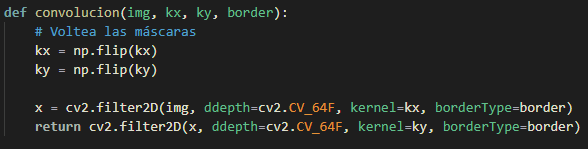
\includegraphics[width=1.0\columnwidth]{conv.png}
% 	\caption{Código convolución}
% \end{figure}

% \newpage

% %------------------------------------------------
% \subsection{Apartado A}
% Se calcula la convolución Gaussiana a partir de las máscaras 1D Gaussianas 
% de OpenCV, pasándolas a la función de convolución.

% Haciendo una exploración de parámetros obtenemos los siguientes resultados:

% \begin{figure}[h]
% 	\centering
% 	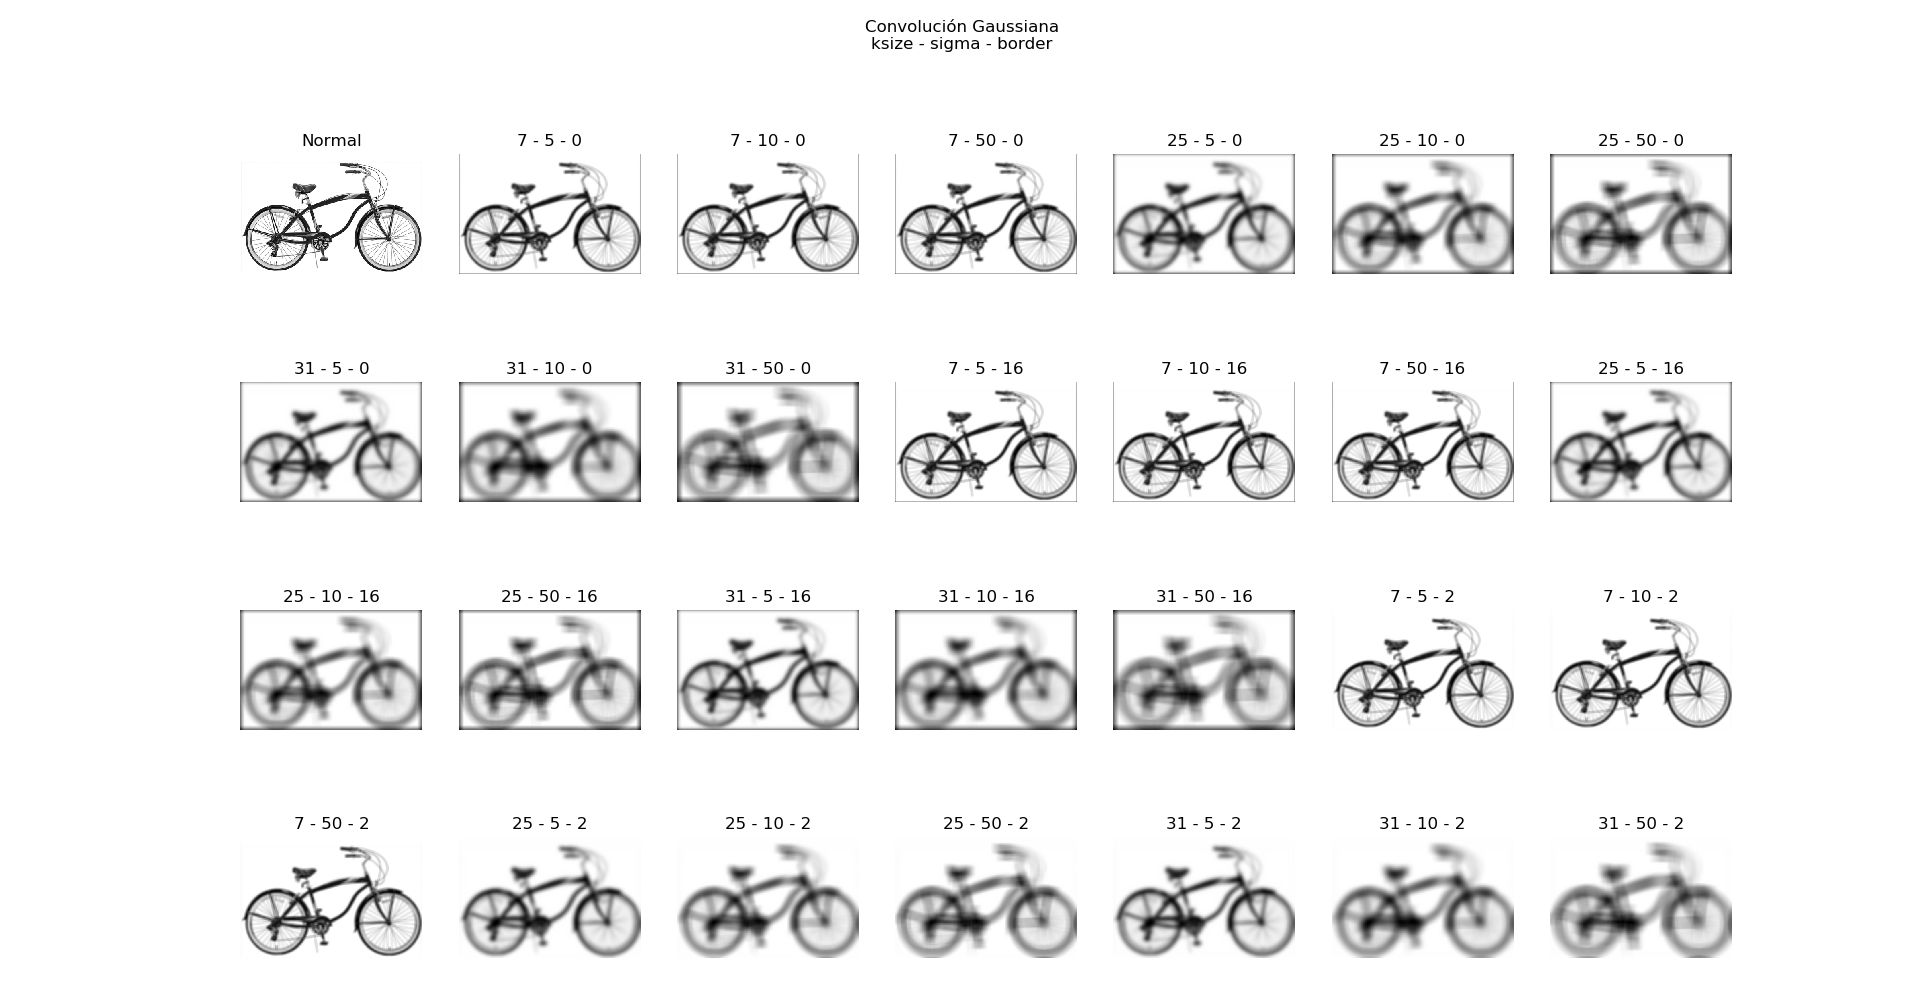
\includegraphics[width=1.0\columnwidth]{1a.png}
% 	\caption{Resultados de convolución Gaussiana}
% \end{figure}

% De lo que se deduce lo siquiente:

% \begin{enumerate}
% 	\item La convolución Gaussiana actua como filtro de paso bajo, elimando 
% 	detalles de la imagen.
% 	\item El tamaño de la máscara y los valores de $\sigma$ son los que determinan el 
% 	grado de suavizado que se aplica (a más alto, más suavizado). Si no se 
% 	incrementa la máscara de manera proporcional a $\sigma$ esta se satura, no
% 	consiguiendo un filtrado mayor por mucho que se aumente.

% 	Por lo aprendido en teoría, el tamaño óptimo de la máscara debe ocupar el rango
% 	[$-3*\sigma$, $+3*\sigma$], es decir, debe ser de $6*\sigma+1$ ($+1$ para 
% 	ser impar).
% 	\item Los diferentes bordes solo se aprecian con máscaras grandes. En la figura
% 	de ejemplo, se aprecia en gran medida el borde constante de 0. En cambio,
% 	por tener el fondo blanco, el borde replicado no se nota.
% \end{enumerate}

% \newpage

% %------------------------------------------------
% \subsection{Apartado B}
% En este caso se implementa el cálculo de una Laplaciana de Gaussiana, realizándole
% primeramente un filtro Gaussiano a la imagen seguido de la aplicación de dos 
% máscaras 1D con las segundas derivadas.


% Haciendo una exploración de parámetros obtenemos los siguientes resultados:

% \begin{figure}[h]
% 	\centering
% 	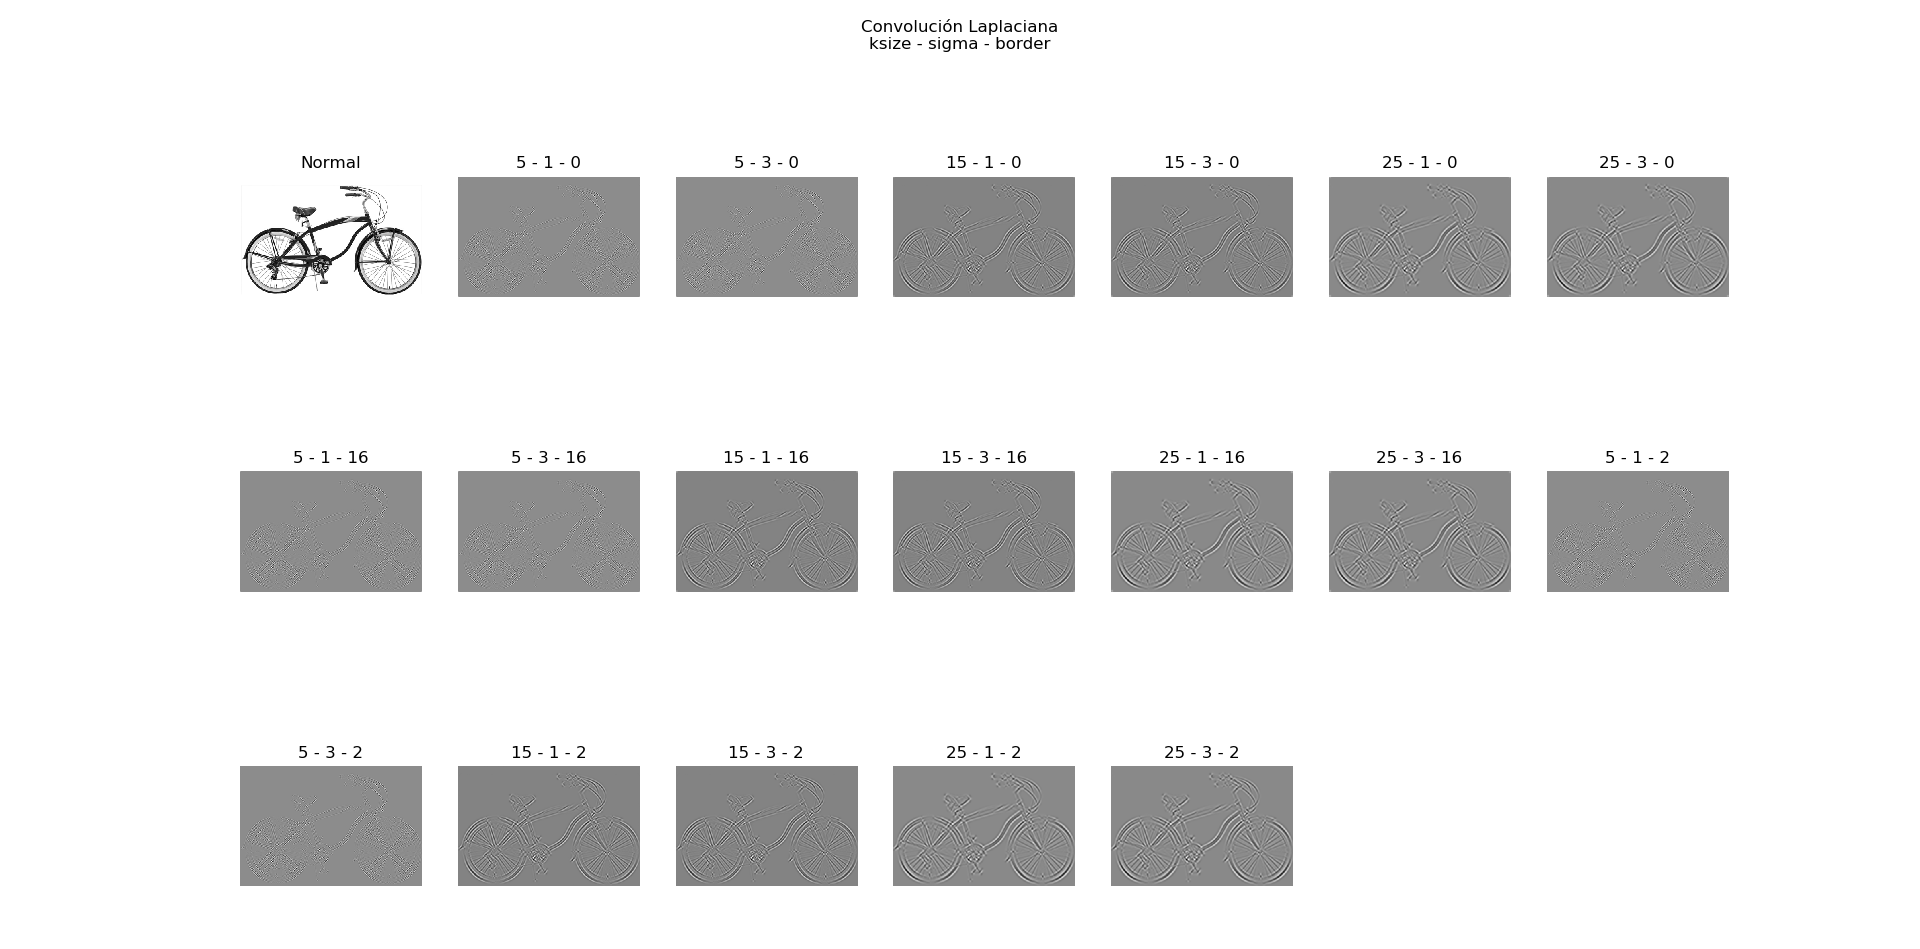
\includegraphics[width=1.0\columnwidth]{1b.png}
% 	\caption{Resultados de convolución Laplaciana}
% \end{figure}

% De lo que se deduce lo siquiente:
% \begin{enumerate}
% 	\item Al estar aplicando derivadas, la Laplaciana de Gaussiana muestra las
% 	regiones de alta frecuencia de la imagen.
% 	\item Puesto que realizamos previamente un filtro gaussiano, los valores de
% 	$\sigma$ y el tamaño de la máscara también son relevantes, consiguiendo detalles
% 	de mayor o menos escala según el grado de suavizado que se aplique previamente.	
% 	\item Al igual que en el apartado anterior, los diferentes bordes solo se 
% 	aprecian con máscaras grandes.
% \end{enumerate}

% \newpage

% %----------------------------------------------------------------------------------------
% %----------------------------------------------------------------------------------------
% %----------------------------------------------------------------------------------------
% %----------------------------------------------------------------------------------------
% \section{Ejercicio 2}

% %------------------------------------------------
% \subsection{Apartado A}
% Partiendo de la función Gaussiana definida en el ejercicio anterior se implementa
% la pirámide. Para ello se aplica un filtro Gaussiano a cada nivel mientras se va
% reduciendo su tamaño.\newline

% Teniendo como ejemplo el siguiente resultado:

% \begin{figure}[h]
% 	\centering
% 	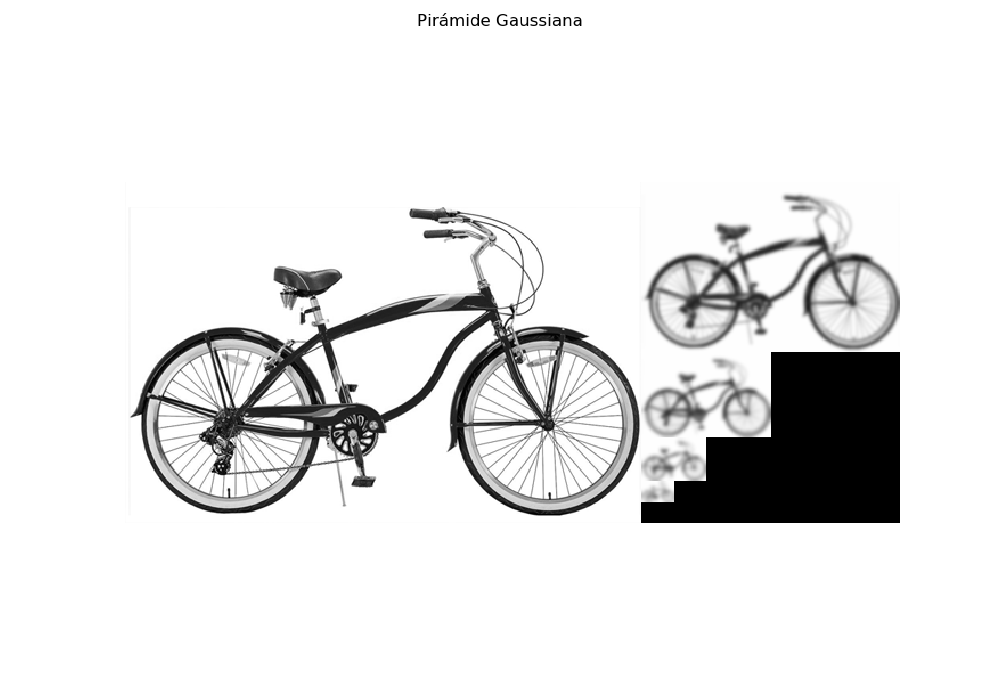
\includegraphics[width=1.0\columnwidth]{2a.png}
% 	\caption{Pirámide Gaussiana}
% \end{figure}

% Se elige un $\sigma=3$ y $ksize=19$ como parámetros ya que se consigue un buen
% suavizado y la máscara ocupa el espacio óptimo de la función Gasusiana 
% [$-3*\sigma$, $+3*\sigma$].


% \newpage

% %------------------------------------------------
% \subsection{Apartado B}
% La función en cada nivel aplica el filtro Gaussiano a la imagen y se lo resta a 
% la original, quedando solo las frecuencias altas, correspondientes a los bordes
% de las figuras.\newline
% Para el último nivel se incluye únicamente la imagen filtrada, ya que nos
% permitiría recuperar la imagen original en caso de que fuera necesario.

% Al igual que en el apartado anterior, se elige un $\sigma=3$ y $ksize=19$ 
% como parámetros ya que se consigue un buen
% suavizado y la máscara ocupa el espacio óptimo de la función Gasusiana 
% [$-3*\sigma$, $+3*\sigma$].\newline

% Al aplicarla se obtiene el siguiente resultado:

% \begin{figure}[h]
% 	\centering
% 	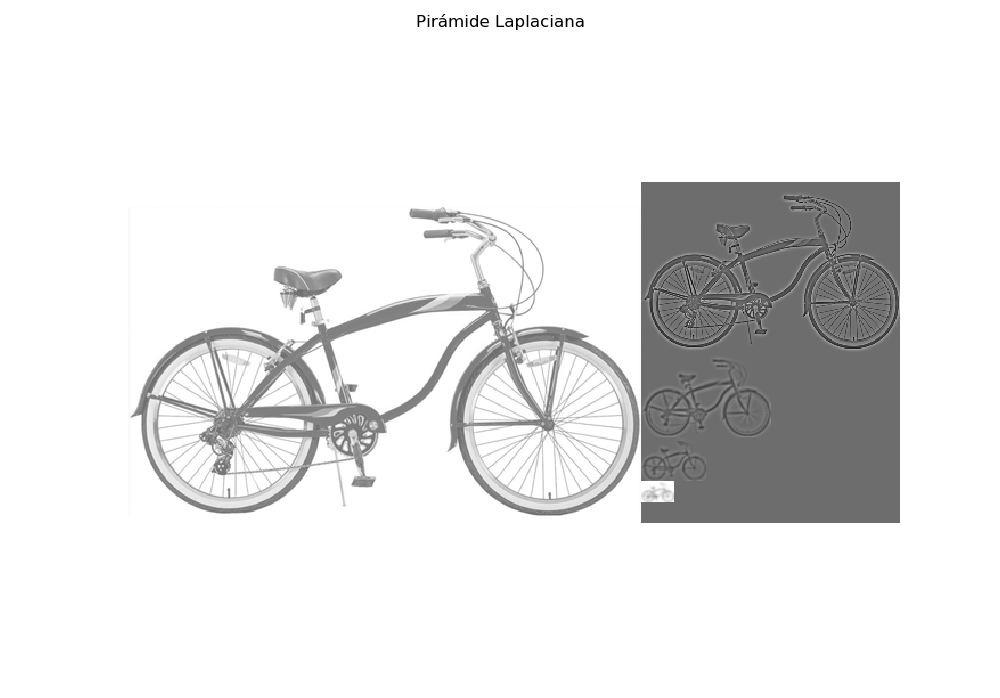
\includegraphics[width=1.0\columnwidth]{2b.png}
% 	\caption{Pirámide Laplaciana}
% \end{figure}

% \newpage

% %------------------------------------------------
% \subsection{Apartado C}

% El espacio de escalas realiza, para cada repetición:
% \begin{enumerate}
% 	\item Filtrado de Laplaciana-Gaussiana a la imagen original.
% 	\item Guardado el cuadrado de las respuestas multiplicados por $\sigma^{2}$.
% 	\item Se le aplica una supresión de no máximos absolutos, guardando el resultado.
% 	\item Se calculan las regiones y se almacenan en una matriz diferente.
% 	\item Se incrementa $\sigma$
% \end{enumerate}

% Se comienzo con $\sigma=1$ para no aplicar demasiado suavizado, se incrementa
% por $1.2$ durante la construcción del espacio, y la máscara tiene el tamaño 
% óptimo según lo mencionado anteriormente.

% \begin{figure}[h]
% 	\centering
% 	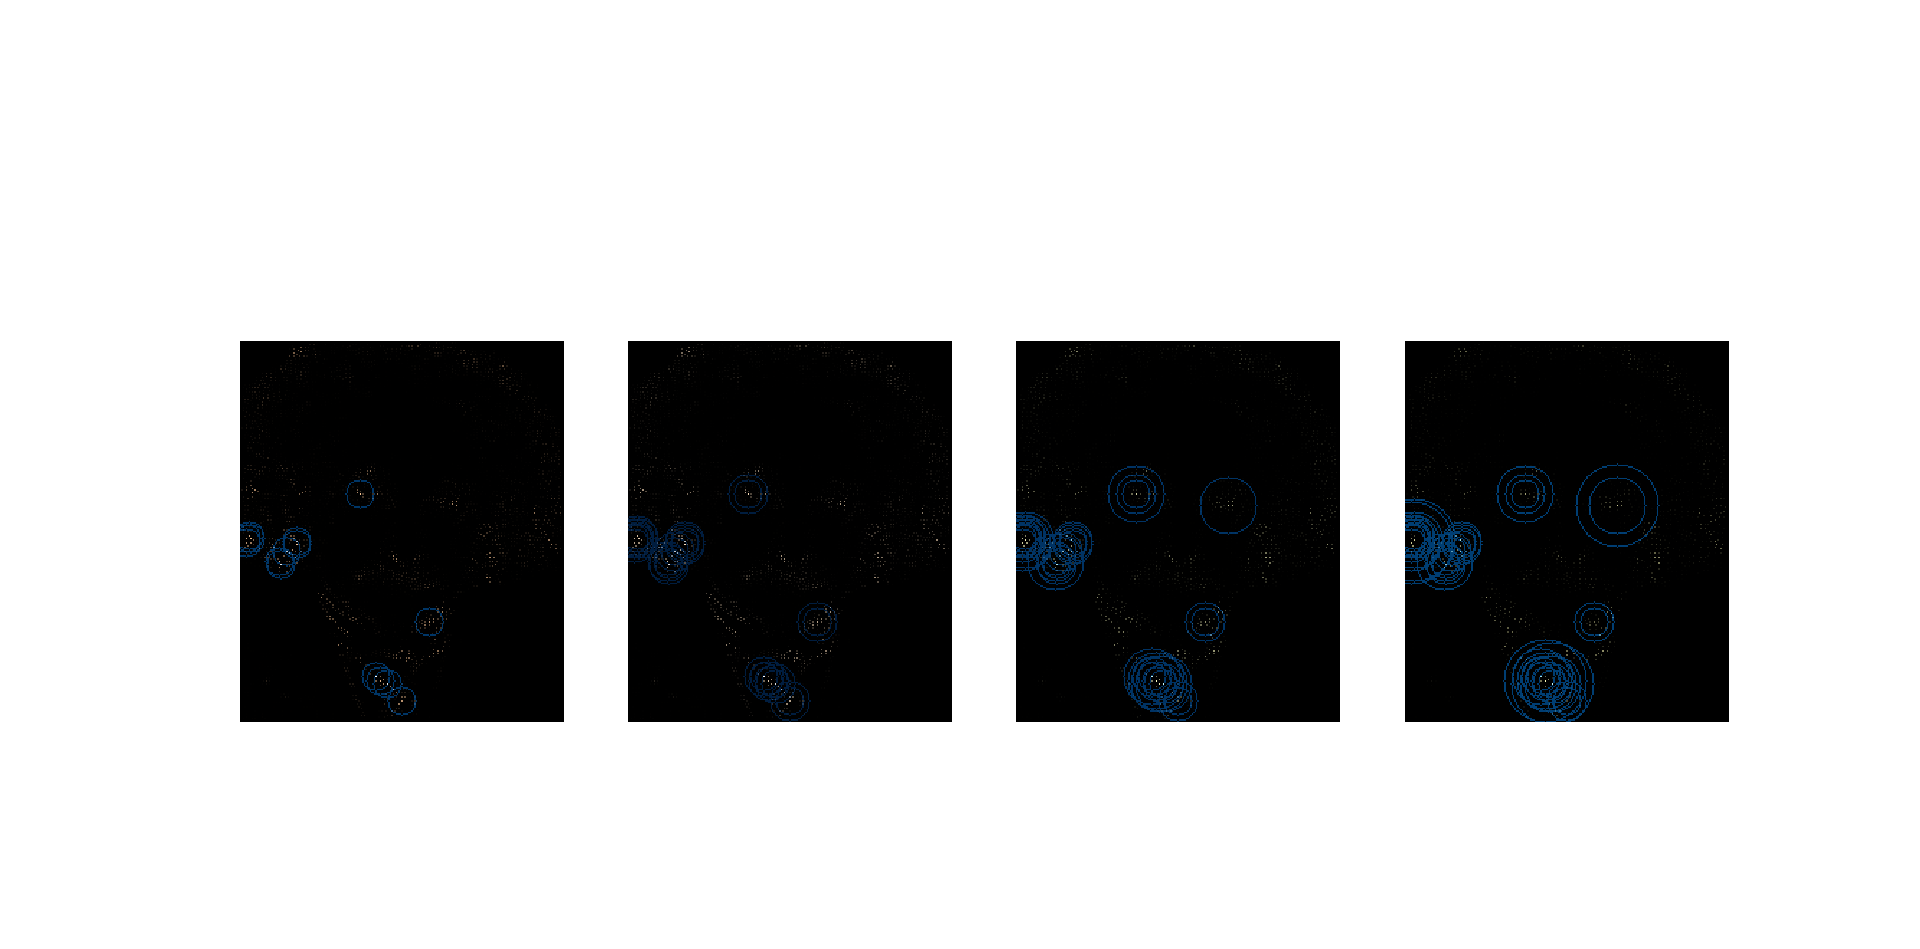
\includegraphics[width=0.8\columnwidth]{2c1.png}
% 	\caption{Regiones detectadas en cada nivel}
% \end{figure}

% \begin{figure}[h]
% 	\centering
% 	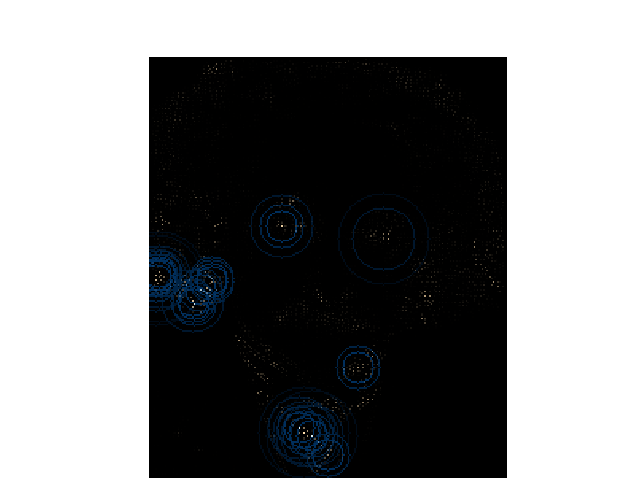
\includegraphics[width=0.8\columnwidth]{2c2.png}
% 	\caption{Regiones detectadas en todos los niveles}
% \end{figure}

% \newpage

% %-------------------------------------------------------------------------------
% %-------------------------------------------------------------------------------
% %-------------------------------------------------------------------------------
% %-------------------------------------------------------------------------------
% \section{Ejercicio 3}

% La función calcula las frecuencias bajas de la primera imagen aplicando un filtro
% Gaussiano, y las altas de la segunda restándole a la imagen original su respectivo
% filtrado Gaussiano.
% Para obtener la imagen híbrida, solamente hay que sumar ambas imágenes.\newline

% Se experimenta individualmente con cada pareja de imágenes hasta conseguir el efecto
% deseado. Para ello se modifican el valor de $\sigma$ y el tamaño de la máscara.
% También se prueba con distintos órdenes ya que algunas imágenes híbridas se ven
% mejor dependiendo de cuál de sus componentes aporta las frecuencias bajas y cuál
% las altas.\newline

% Se aprecia que subiendo el valor de $\sigma$ en la imagen de baja frecuencia se
% consigue que sea menos apreciable.
% Por el contrario, si es muy baja o si se sube demasiado en las de alta frecuencia
% esta se ve demasiado. \newline

% Vemos que se consigue el efecto deseado al mostrar la pirámide Gaussiana, ya que
% simula el efecto de alejarse de la imagen:

% \begin{enumerate}
% 	\item Con la primera pareja notamos como la "sombra" de la motocicleta acaba usurpando
% 	a la bicicleta.
% 	\item Con la segunda los detalles de la cara de Einstein acaban convirtiendose en los 
% 	difusos de Marilyn.
% 	\item Y en la tercera en especial se nota la diferencia en los ojos que nos cambia la
% 	percepción entre una imagen y otra.
% \end{enumerate}

% \begin{figure}[h]
% 	\centering
% 	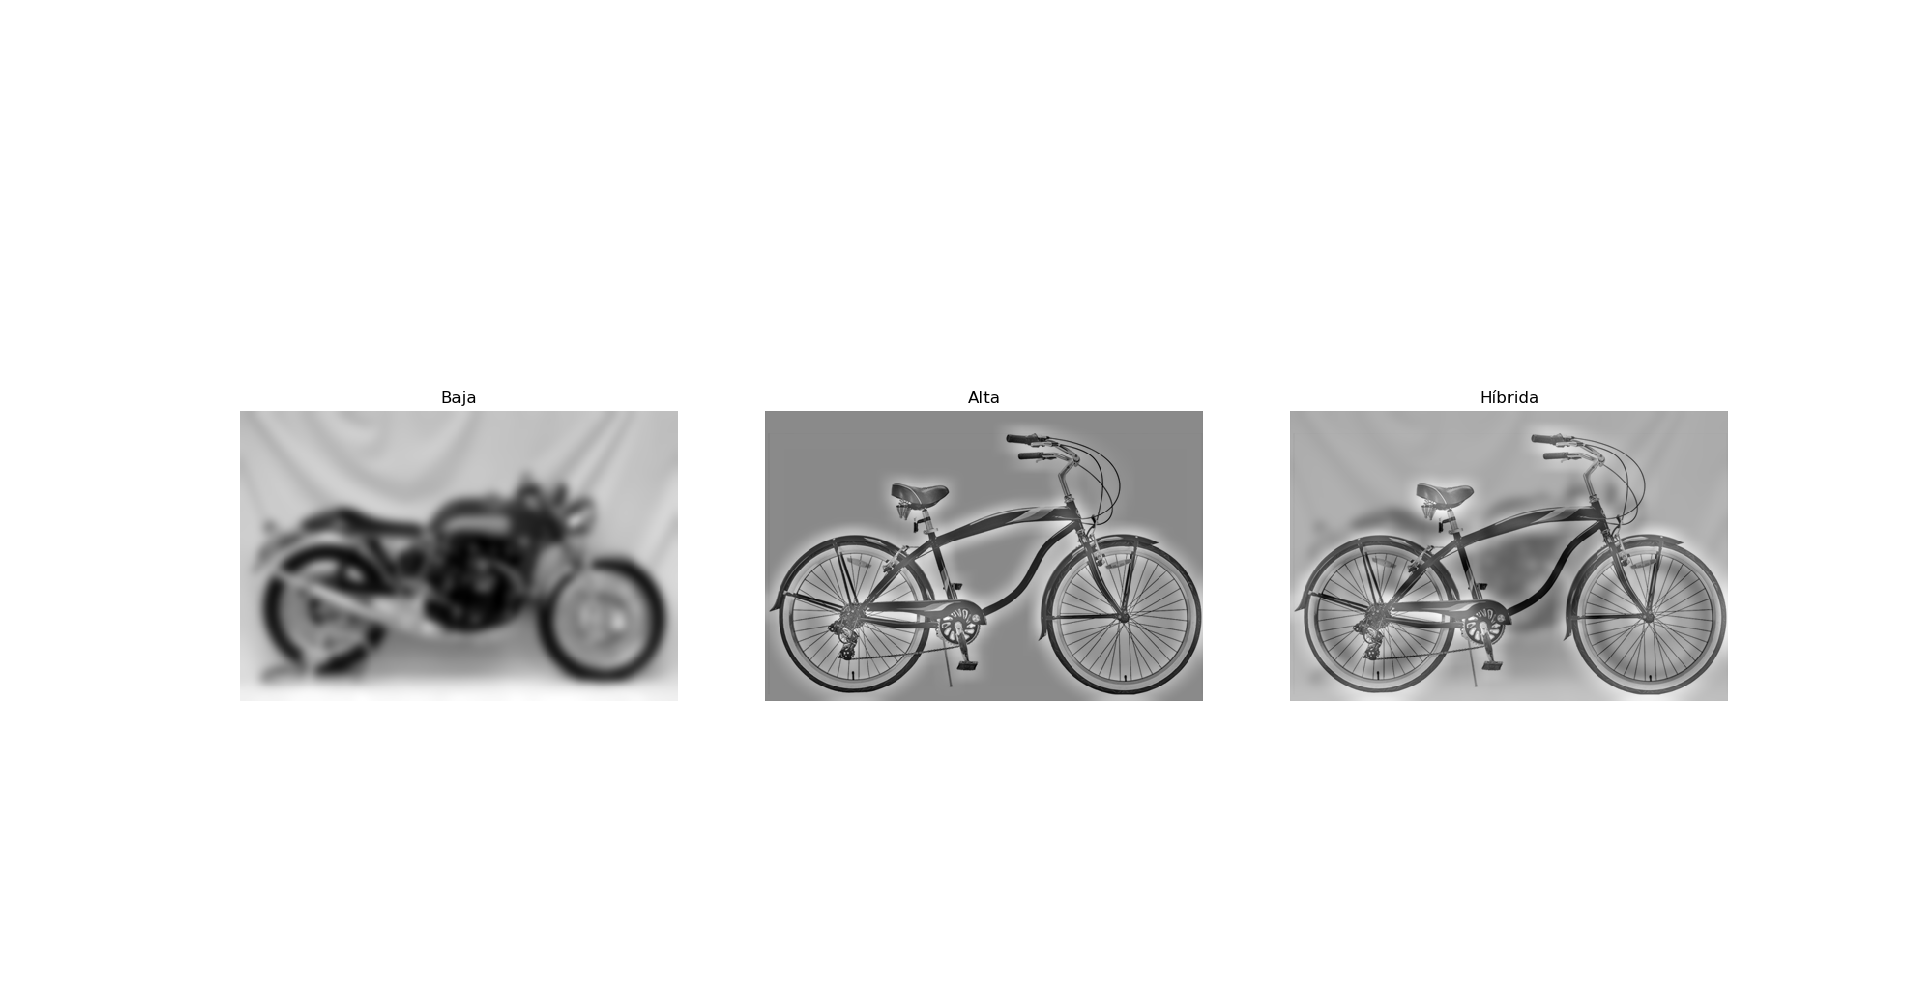
\includegraphics[width=1.0\columnwidth]{31a.png}
% 	\caption{Imágenes baja/alta frecuencia e híbrida, primera pareja}
% \end{figure}

% \begin{figure}[h]
% 	\centering
% 	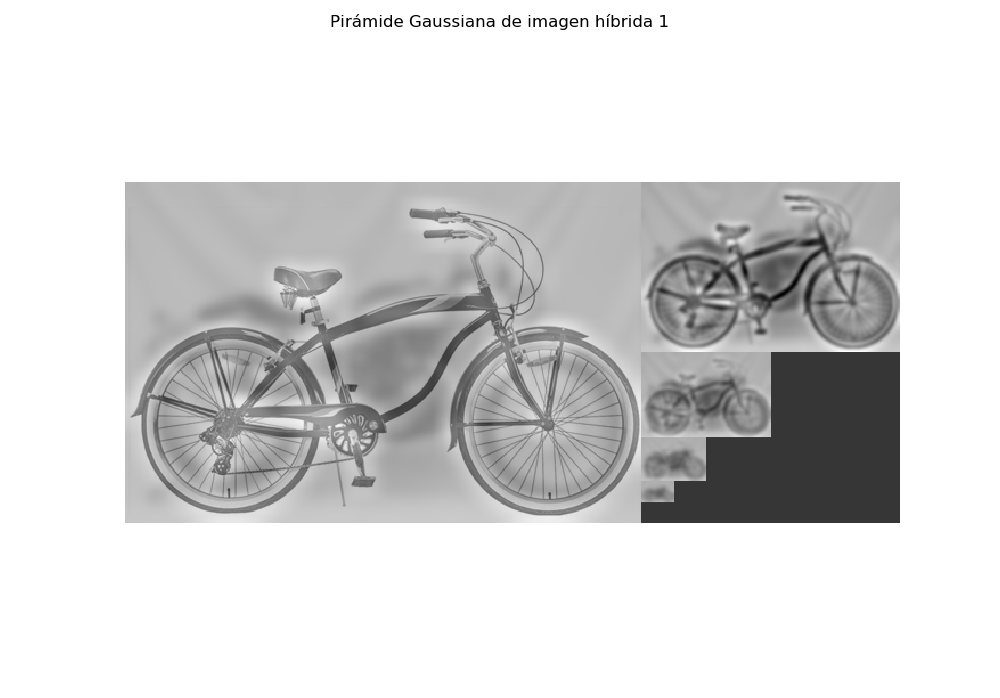
\includegraphics[width=1.0\columnwidth]{31b.png}
% 	\caption{Pirámide Gaussiana de imágen híbrida, primera pareja}
% \end{figure}


% \begin{figure}[h]
% 	\centering
% 	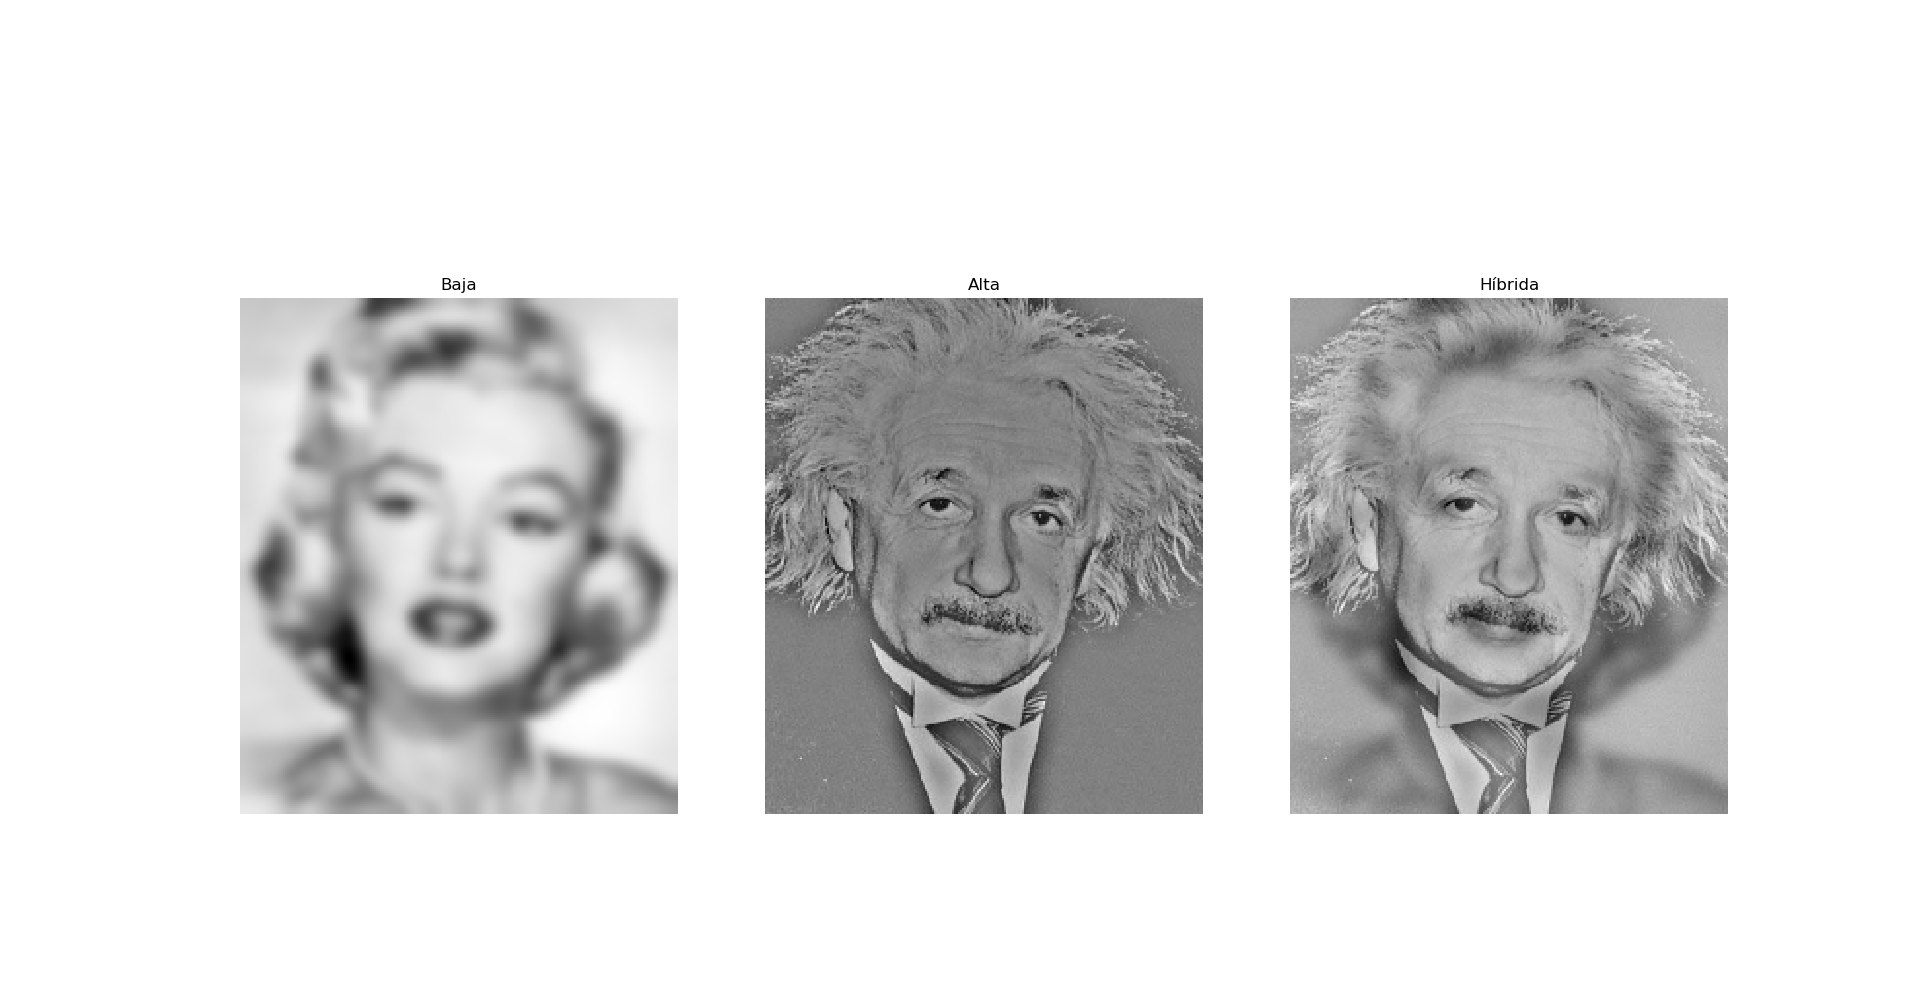
\includegraphics[width=1.0\columnwidth]{32a.png}
% 	\caption{Imágenes baja/alta frecuencia e híbrida, segunda pareja}
% \end{figure}

% \begin{figure}[h]
% 	\centering
% 	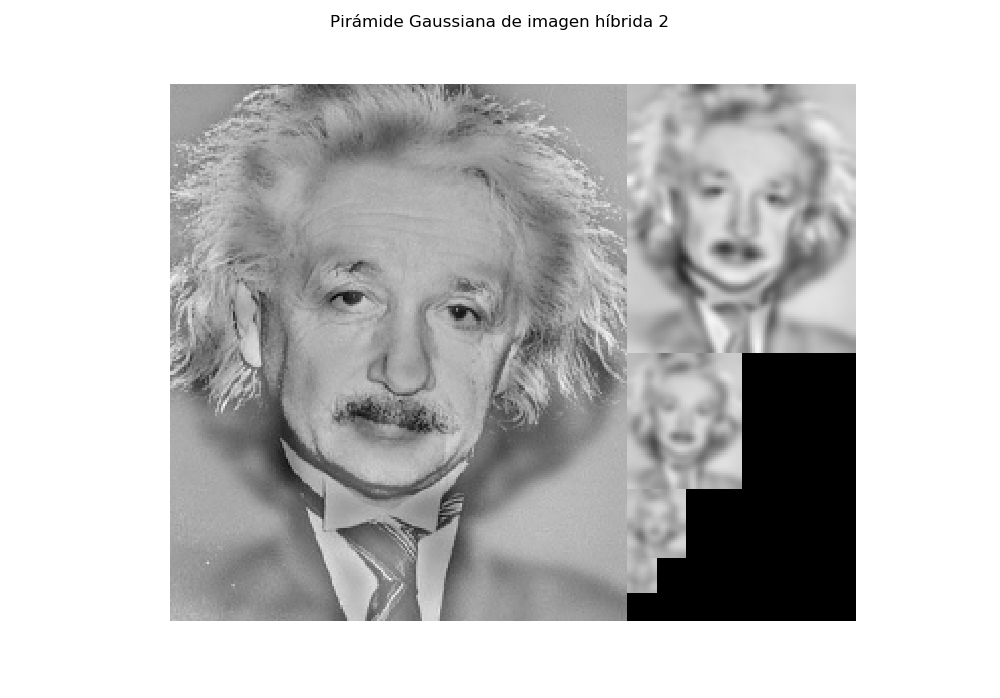
\includegraphics[width=1.0\columnwidth]{32b.png}
% 	\caption{Pirámide Gaussiana de imágen híbrida, segunda pareja}
% \end{figure}


% \begin{figure}[h]
% 	\centering
% 	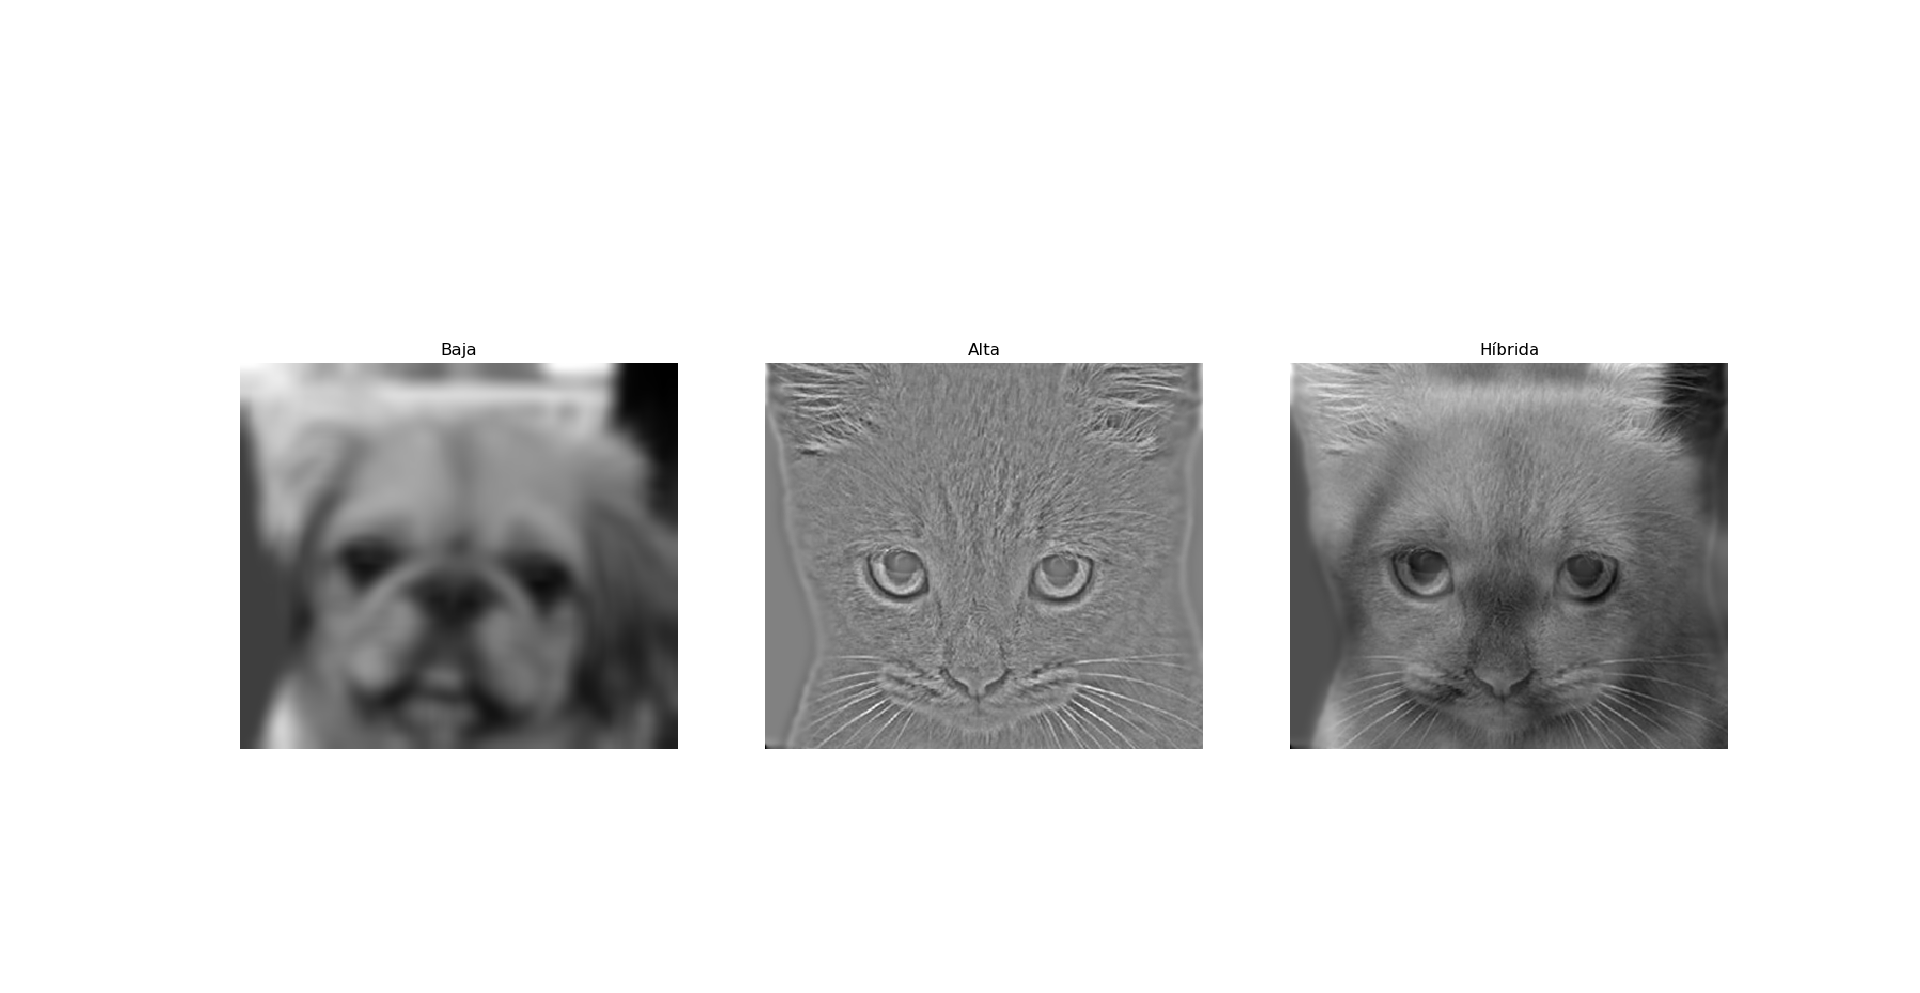
\includegraphics[width=1.0\columnwidth]{33a.png}
% 	\caption{Imágenes baja/alta frecuencia e híbrida, tercera pareja}
% \end{figure}

% \begin{figure}[h]
% 	\centering
% 	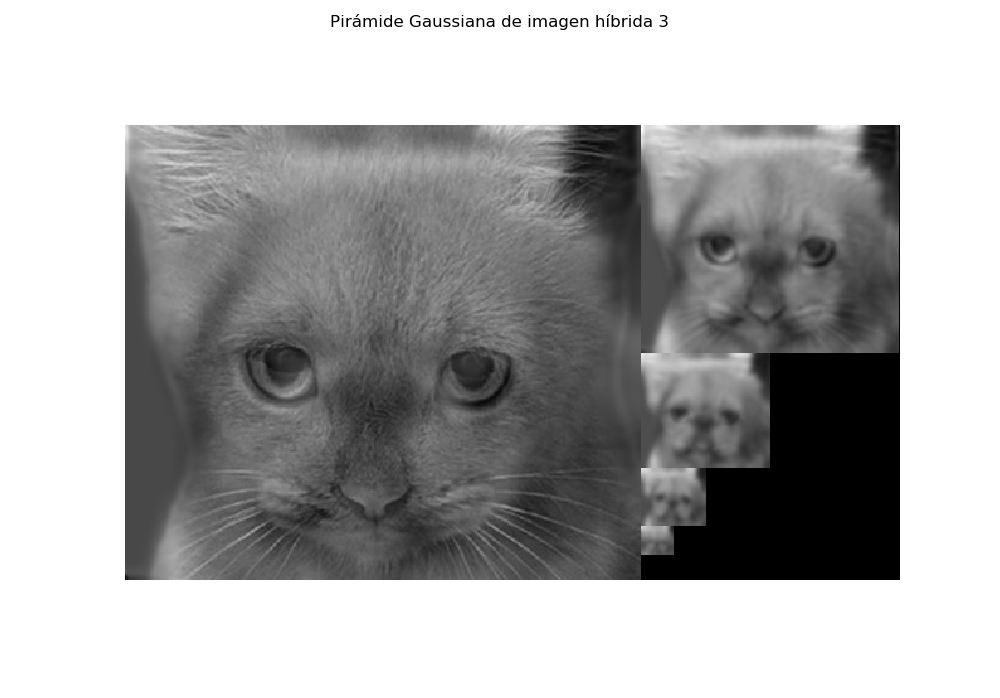
\includegraphics[width=1.0\columnwidth]{33b.png}
% 	\caption{Pirámide Gaussiana de imágen híbrida, tercera pareja}
% \end{figure}

%-------------------------------------------------------------------------------
%-------------------------------------------------------------------------------
%-------------------------------------------------------------------------------
%-------------------------------------------------------------------------------
% \section{Bonus 1}

% Se implementa la convolución a mano con máscaras 1D, para ello:

% \begin{enumerate}
% 	\item Se voltean las máscaras.
% 	\item Se normalizan.
% 	\item Se crea una nueva imagen destino, y se amplía la imagen original con
% 	un borde de ceros.
% 	\item Para cada canal, y para cada elemento de la imagen original, se calcula
% 	su vecindario según el tamaño de las máscaras y se aplican estas, calculando
% 	el valor del pixel en la imagen convolucionada.
% \end{enumerate}

% \begin{figure}[h]
% 	\centering
% 	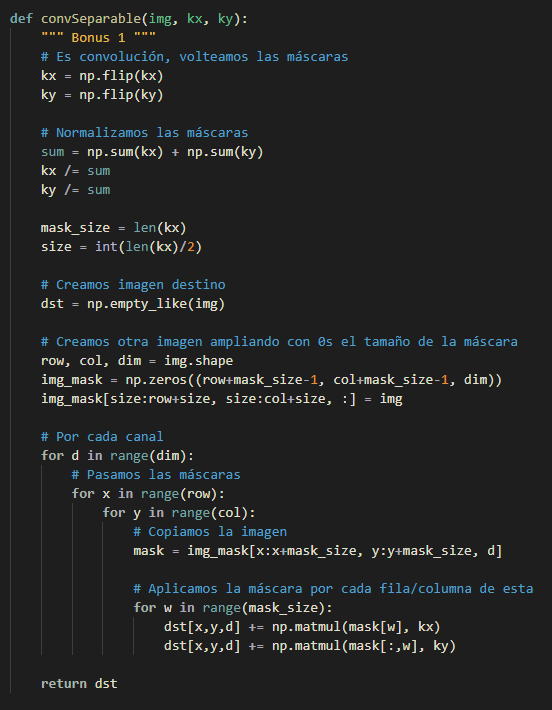
\includegraphics[width=0.7\columnwidth]{convsep1.png}
% 	\caption{Código convolución separable}
% \end{figure}

% \newpage

% Comparando con una imagen Gaussiana, vemos que el resultado es correcto:

% \begin{figure}[h]
% 	\centering
% 	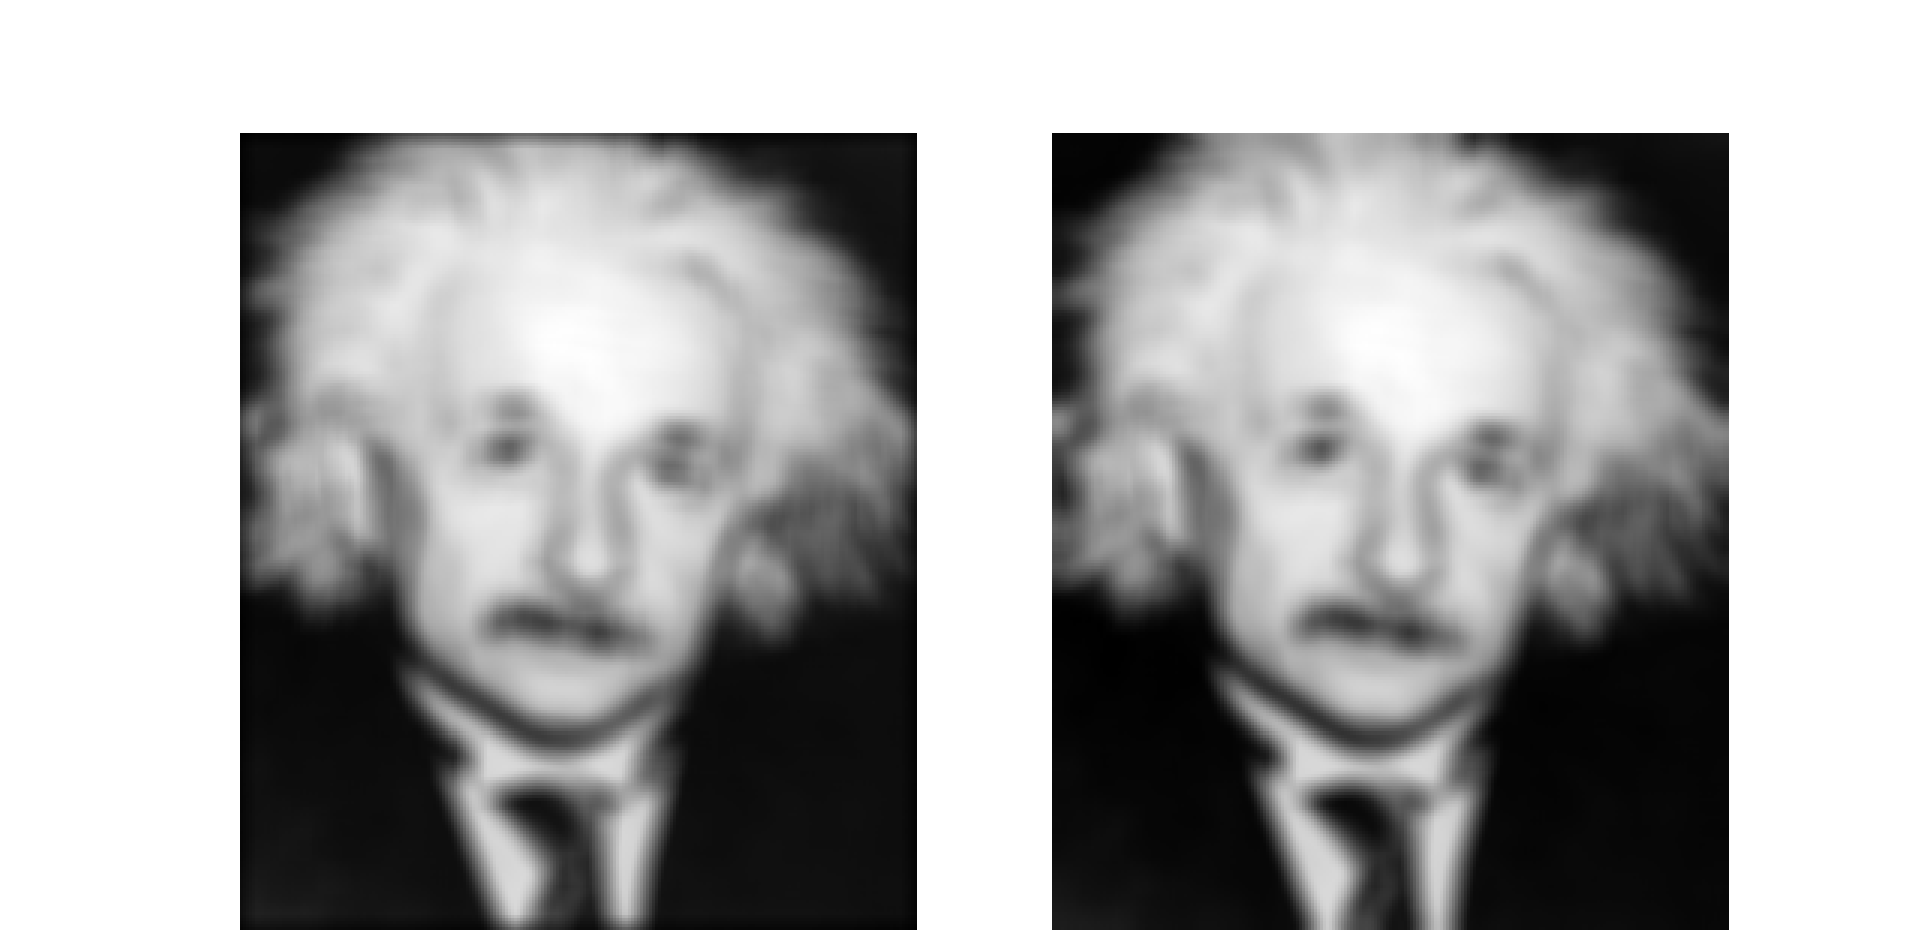
\includegraphics[width=1.0\columnwidth]{convsep2.png}
% 	\caption{Ejemplo convolución separable}
% \end{figure}


%-------------------------------------------------------------------------------
%-------------------------------------------------------------------------------
%-------------------------------------------------------------------------------
%-------------------------------------------------------------------------------
% \vspace{5em}
% \section{Bonus 2}

% Se utiliza las mismas funciones que en el ejercicio 3.\newline

% Para las nuevas imagenes fue necesario volver a probar con distintos parámetros y
% órdenes hasta conseguir el efecto deseado.\newline

% Algunas imágenes no combinan bien a color, como es el caso de la primera pareja.
% Esto se debe a que los objetos no ocupan exactamente la misma parte del espacio,
% y por tanto son capaces de distinguirse a la distancia que no le corresponde.

% \begin{figure}[h]
% 	\centering
% 	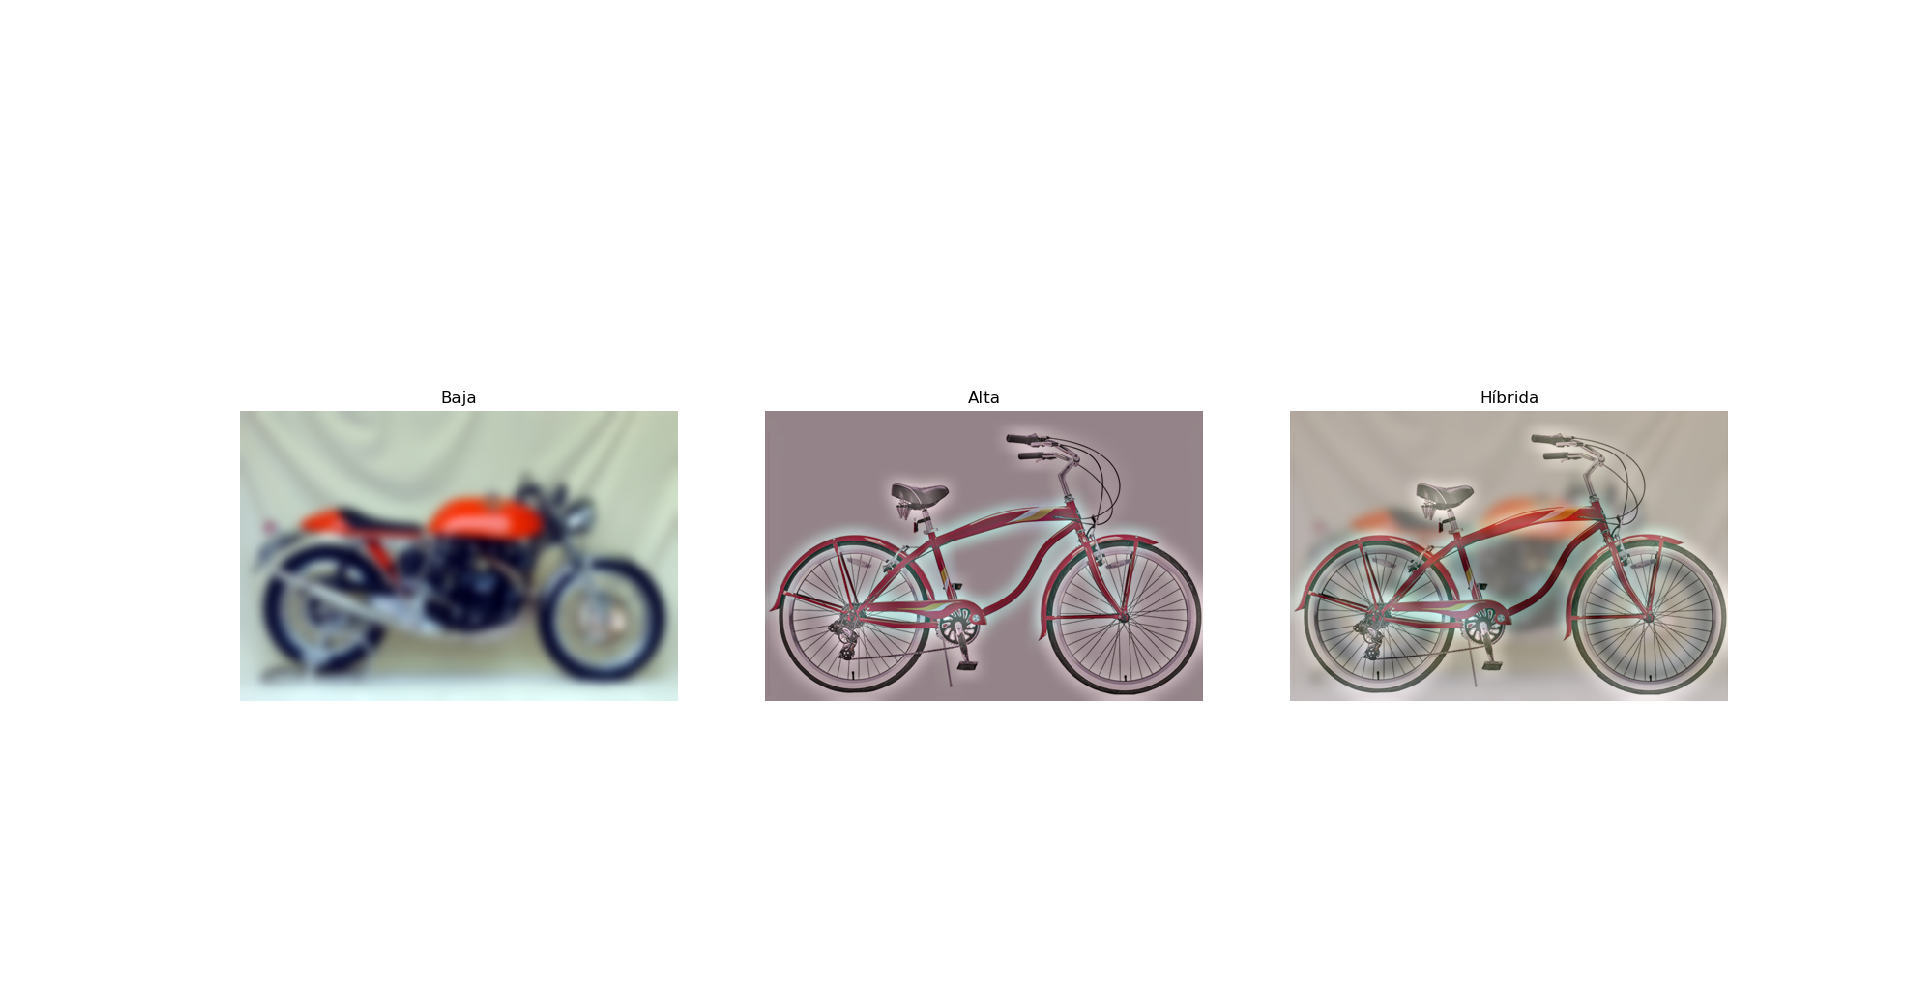
\includegraphics[width=1.0\columnwidth]{b21a.png}
% 	\caption{Imágenes baja/alta frecuencia e híbrida}

% 	\centering
% 	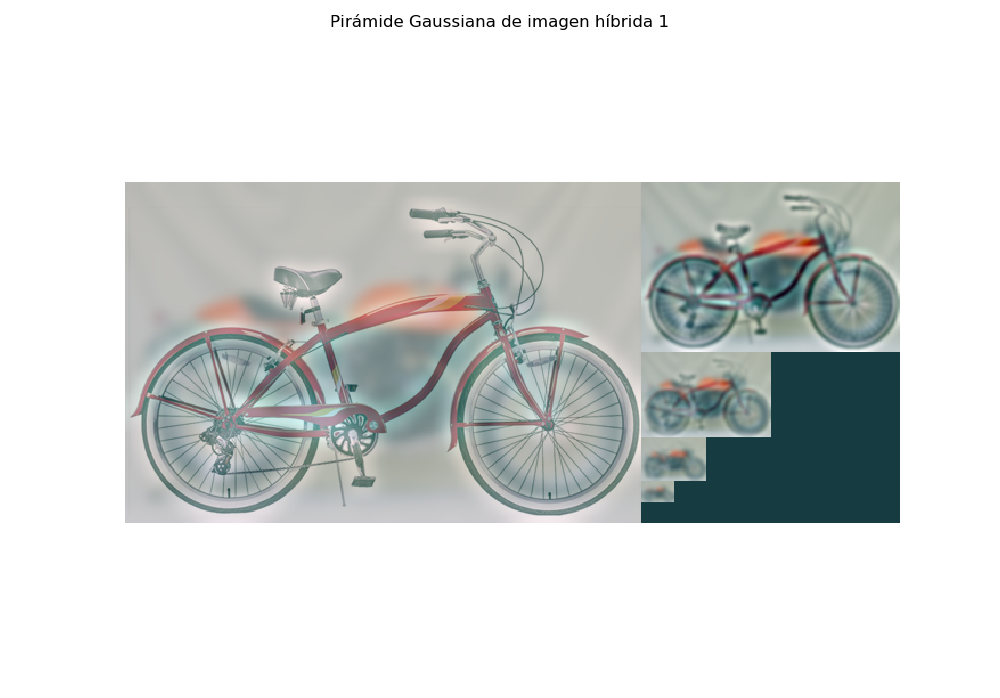
\includegraphics[width=1.0\columnwidth]{b21b.png}
% 	\caption{Pirámide Gaussiana de imágen híbrida}
% \end{figure}

% \begin{figure}[h]
% 	\centering
% 	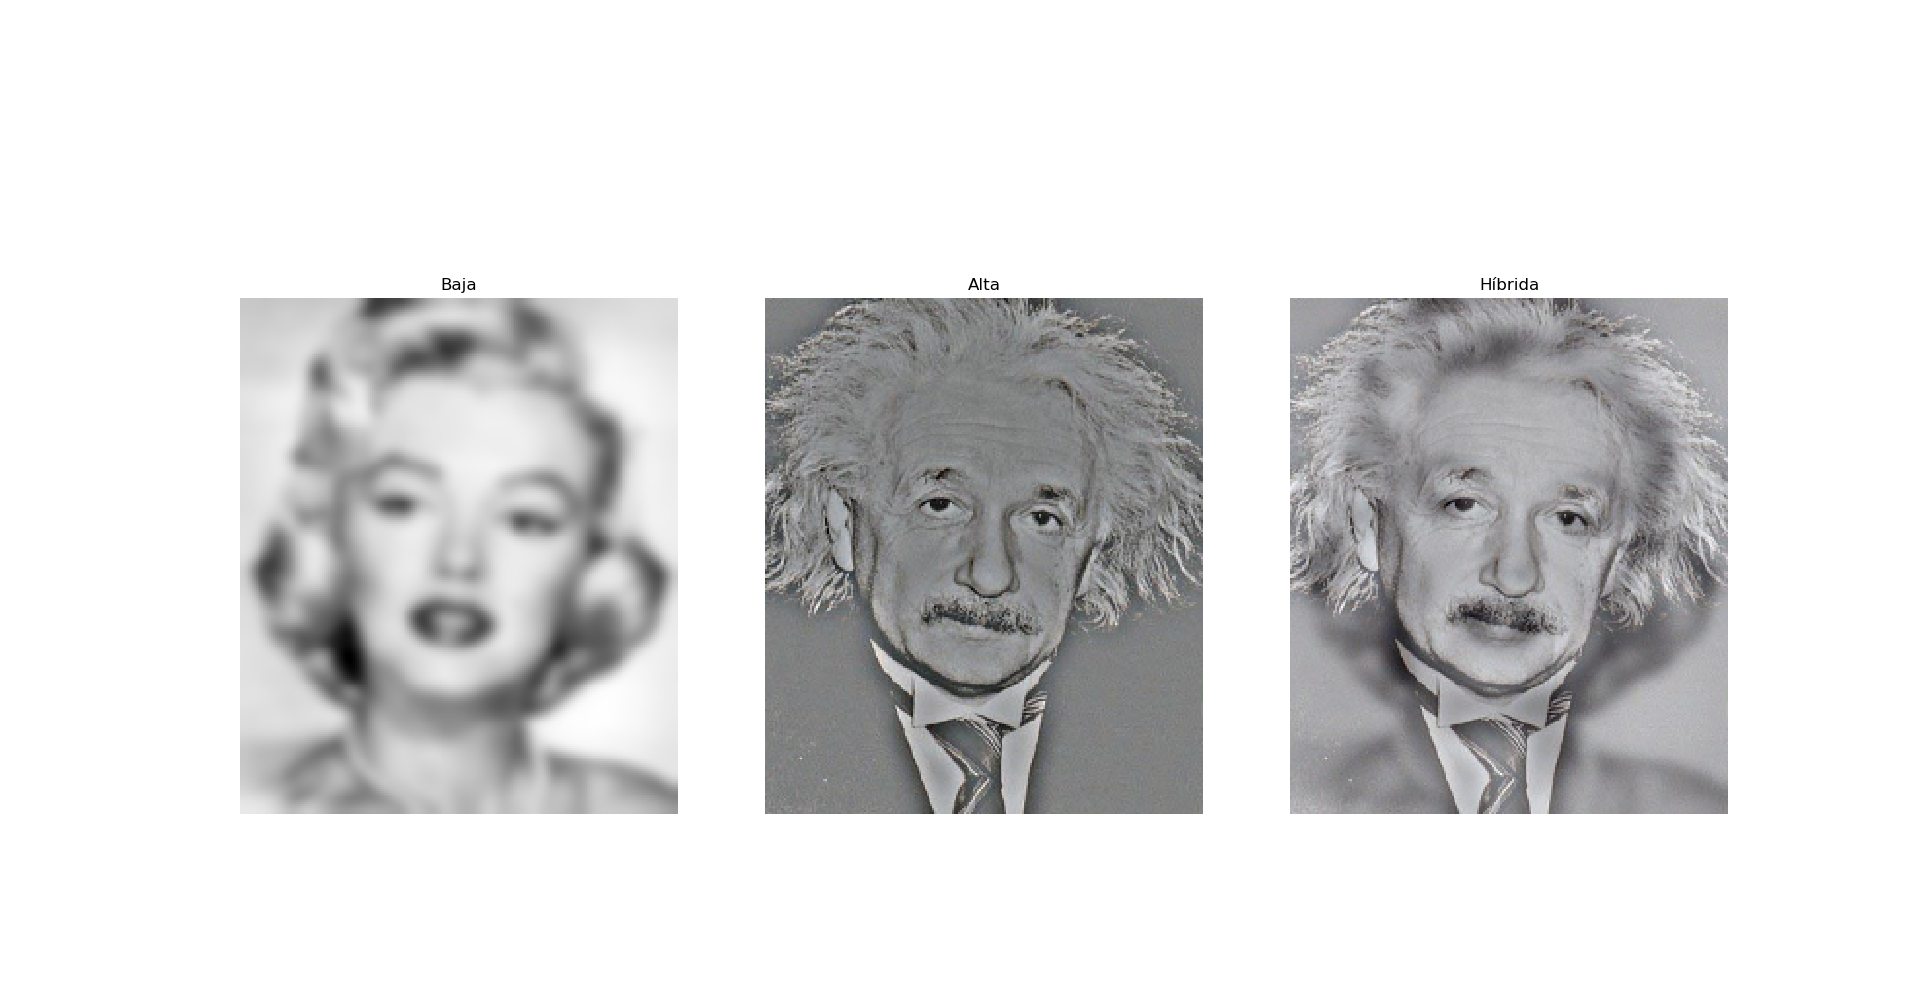
\includegraphics[width=1.0\columnwidth]{b22a.png}
% 	\caption{Imágenes baja/alta frecuencia e híbrida}

% 	\centering
% 	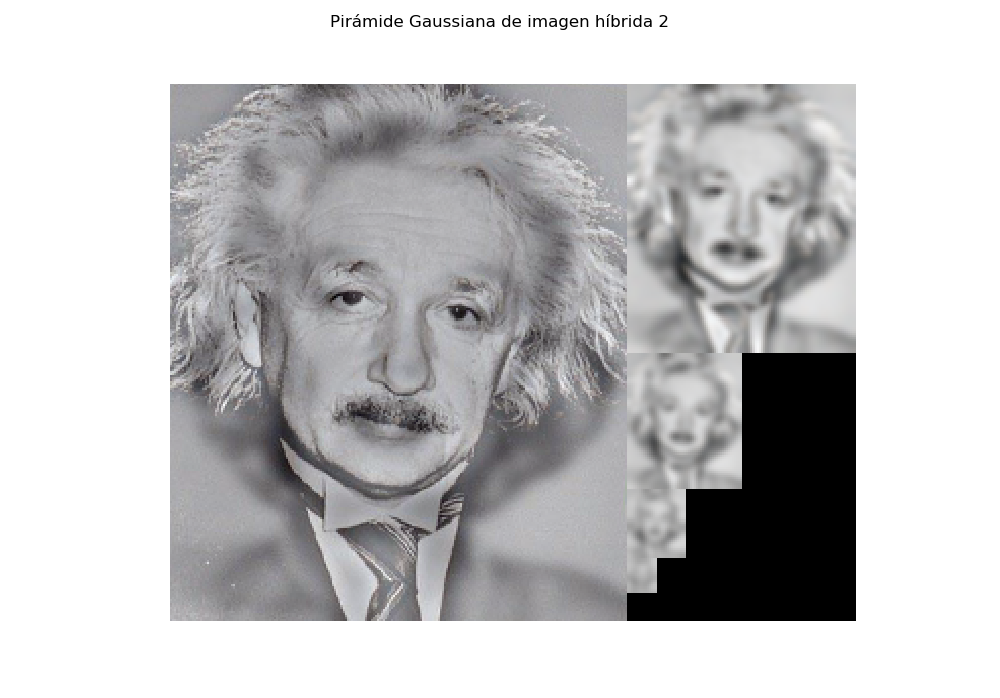
\includegraphics[width=1.0\columnwidth]{b22b.png}
% 	\caption{Pirámide Gaussiana de imágen híbrida}
% \end{figure}

% \begin{figure}[h]
% 	\centering
% 	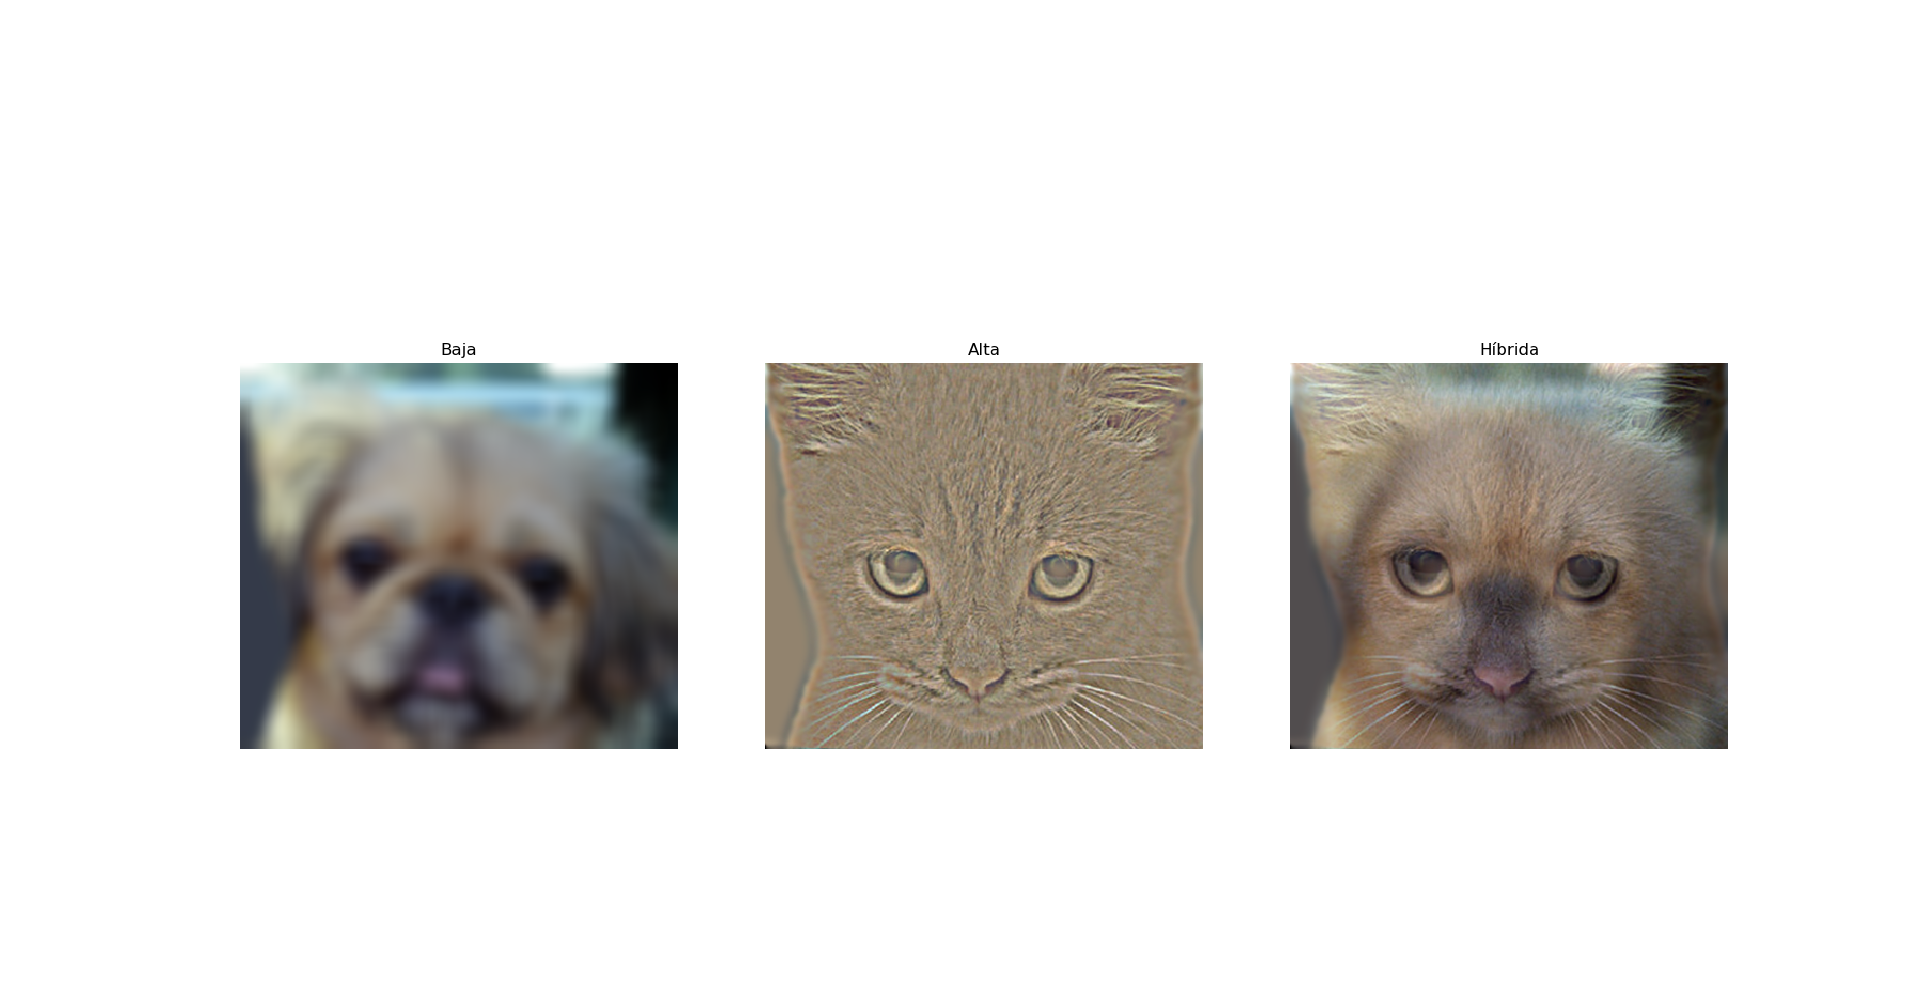
\includegraphics[width=1.0\columnwidth]{b23a.png}
% 	\caption{Imágenes baja/alta frecuencia e híbrida}

% 	\centering
% 	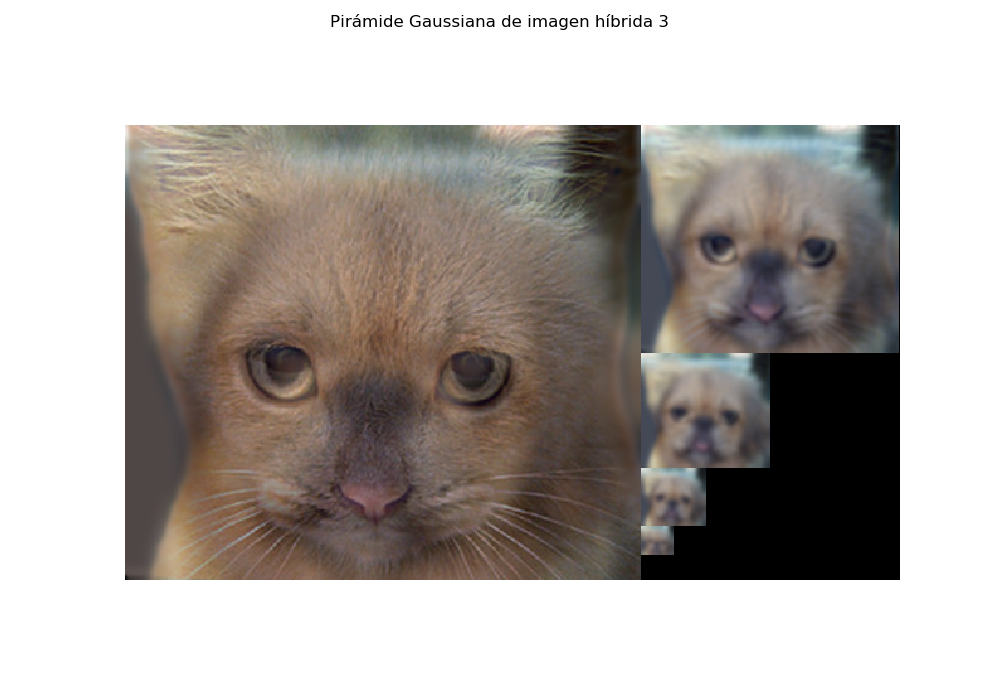
\includegraphics[width=1.0\columnwidth]{b23b.png}
% 	\caption{Pirámide Gaussiana de imágen híbrida}
% \end{figure}

% \begin{figure}[h]
% 	\centering
% 	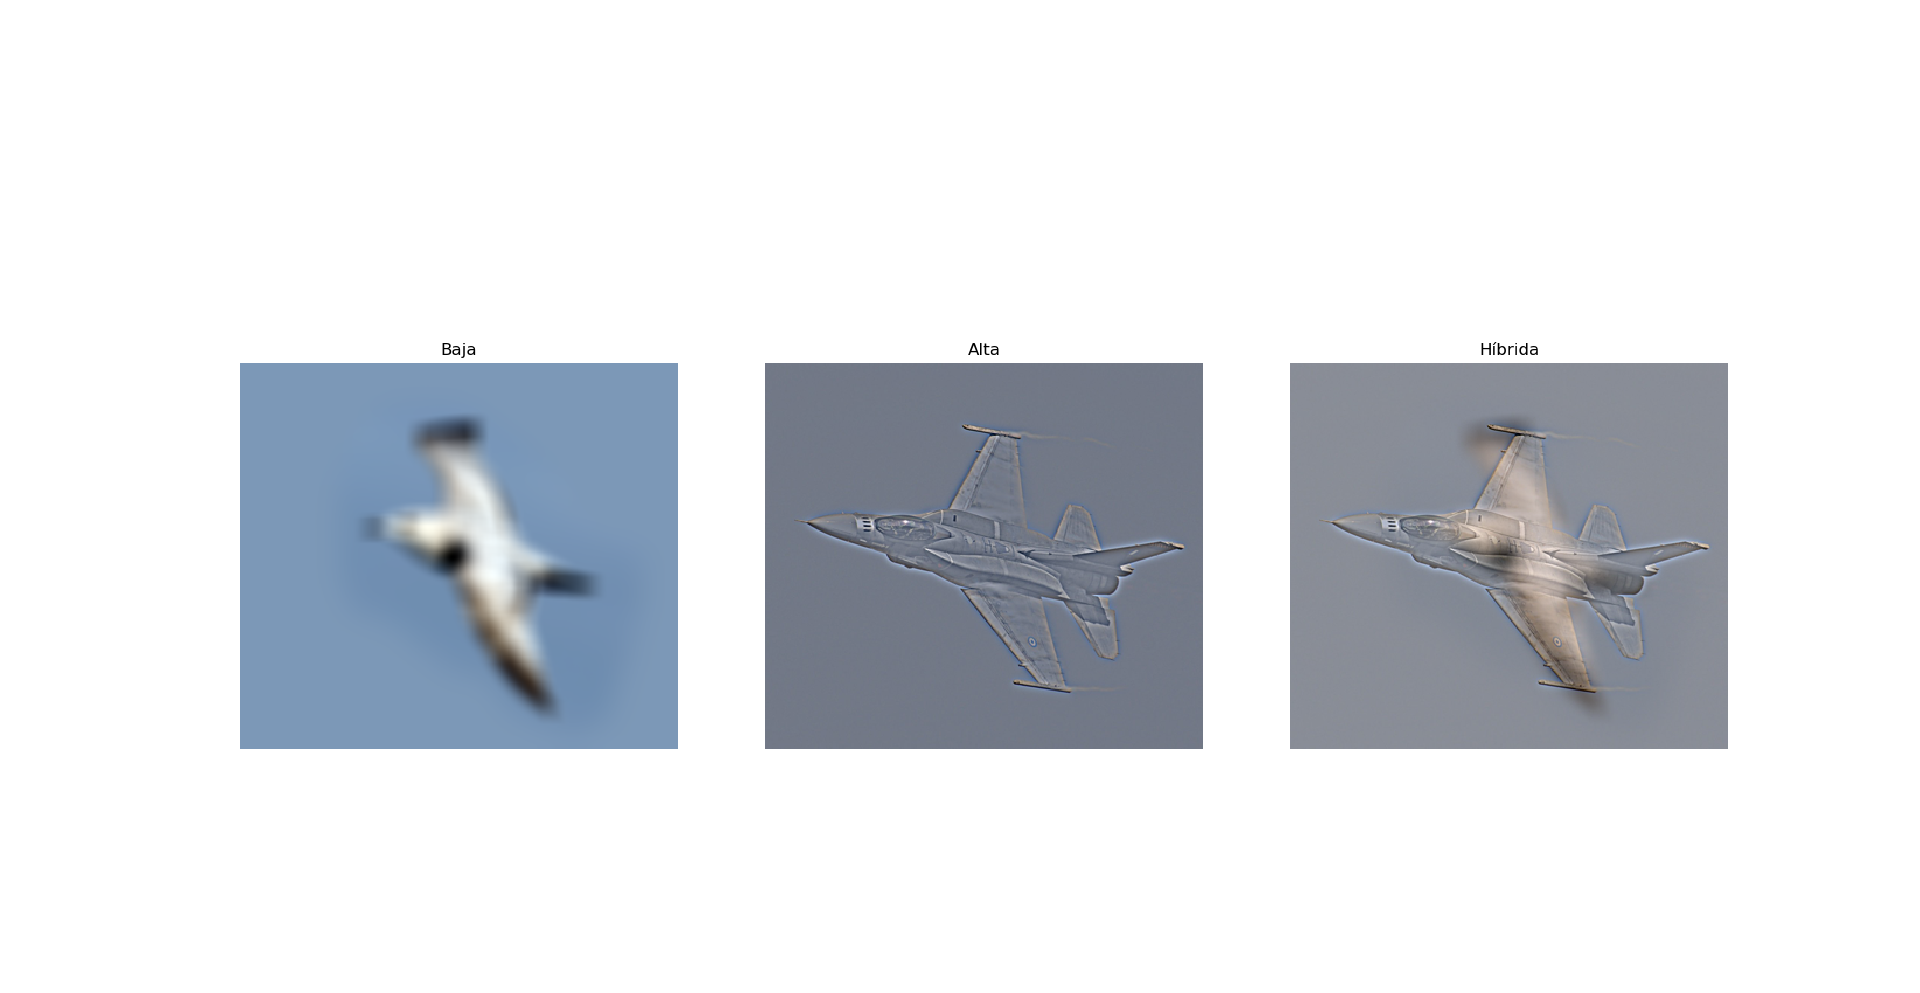
\includegraphics[width=1.0\columnwidth]{b24a.png}
% 	\caption{Imágenes baja/alta frecuencia e híbrida}

% 	\centering
% 	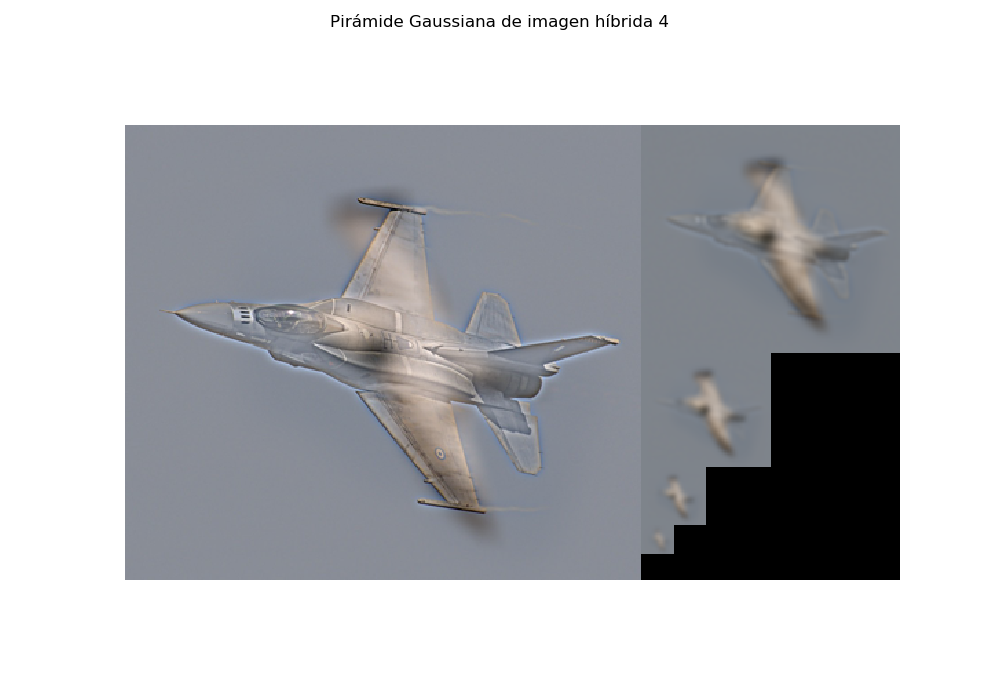
\includegraphics[width=1.0\columnwidth]{b24b.png}
% 	\caption{Pirámide Gaussiana de imágen híbrida}
% \end{figure}

% \begin{figure}[h]
% 	\centering
% 	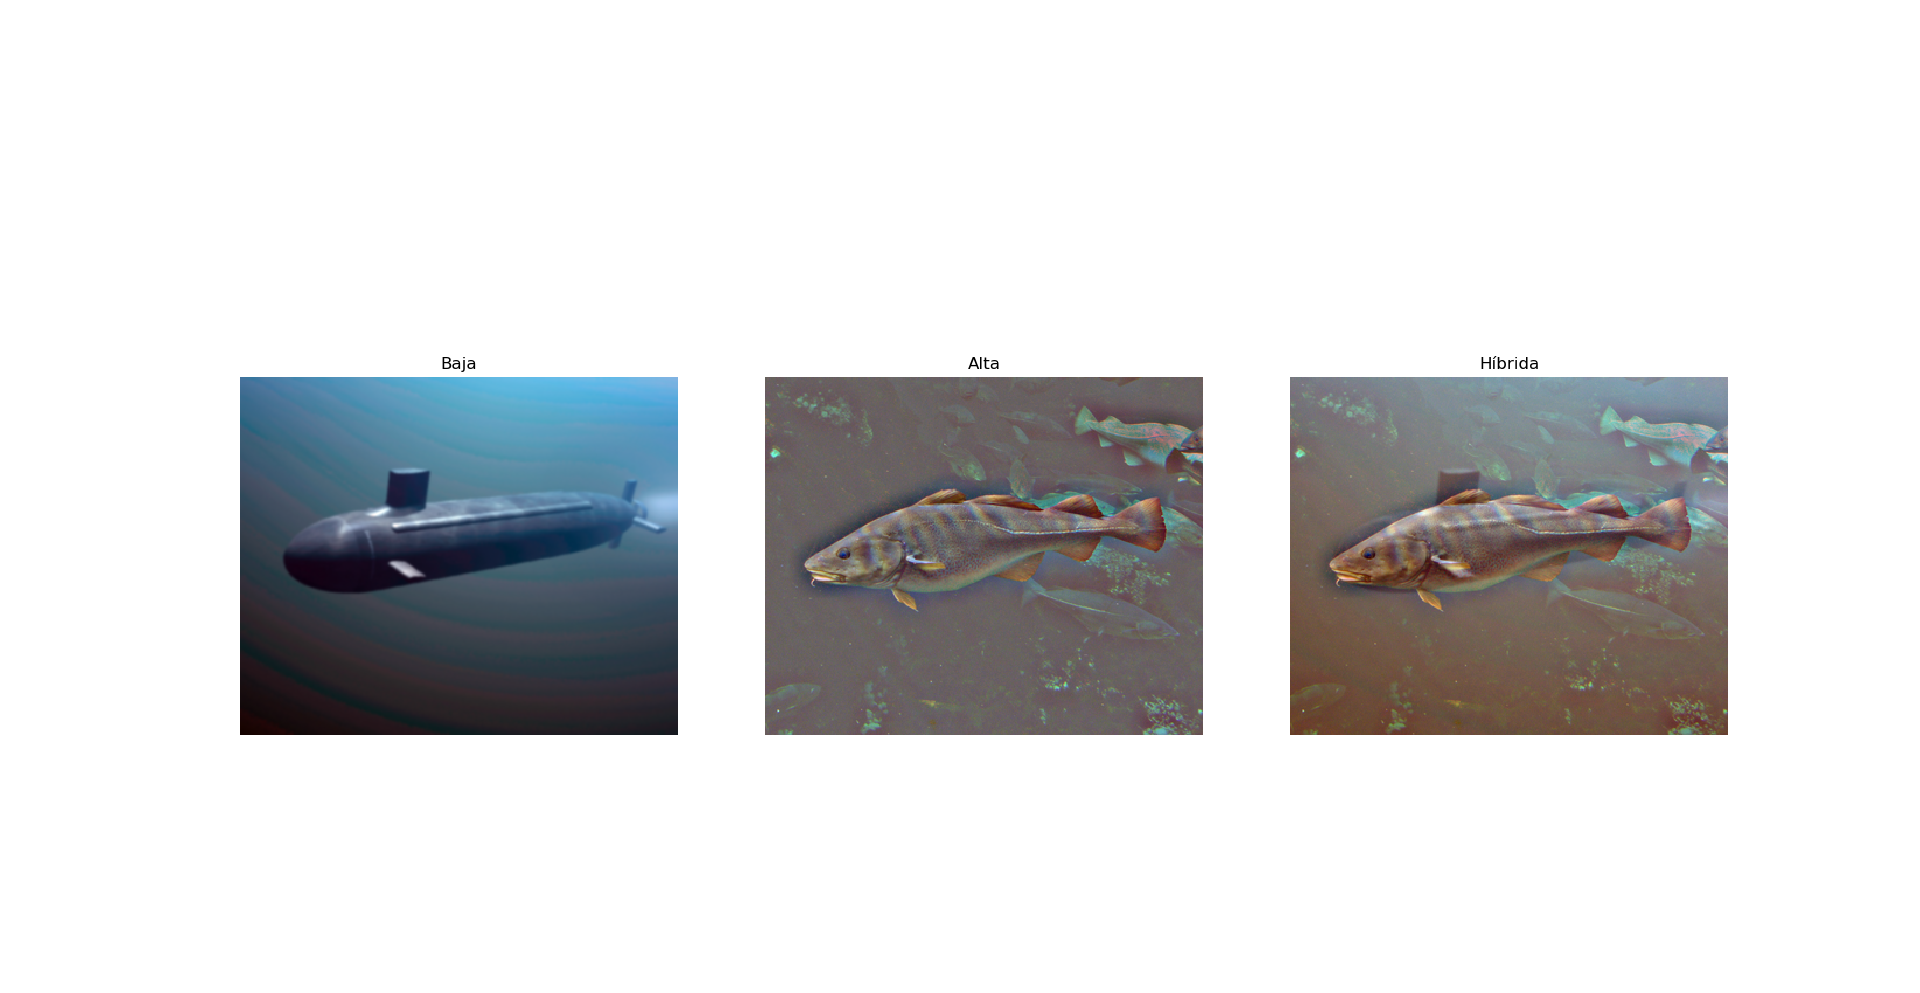
\includegraphics[width=1.0\columnwidth]{b25a.png}
% 	\caption{Imágenes baja/alta frecuencia e híbrida}

% 	\centering
% 	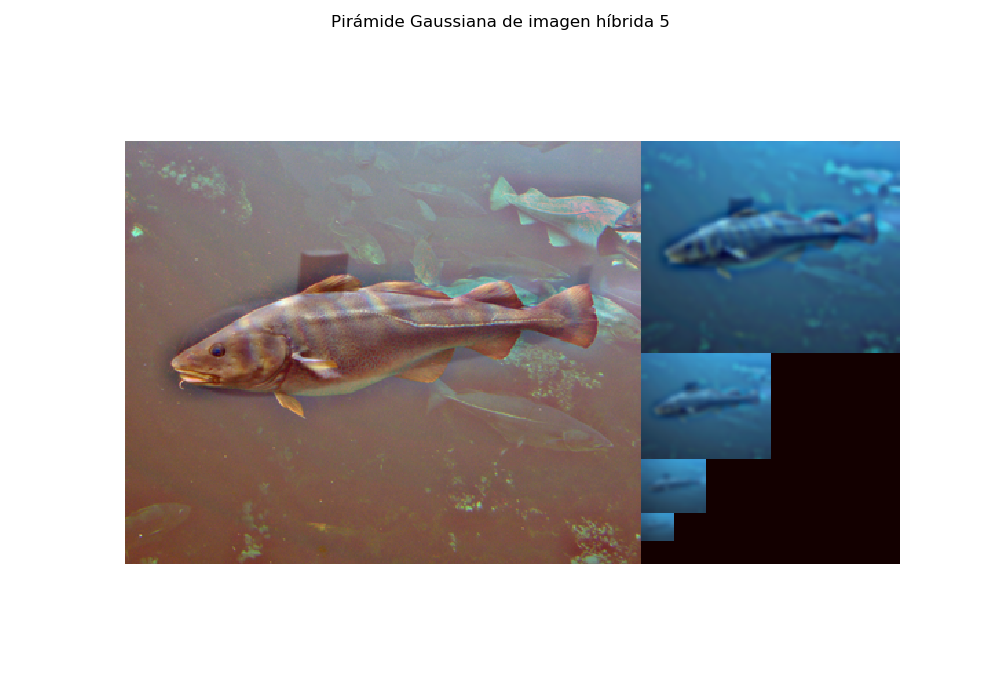
\includegraphics[width=1.0\columnwidth]{b25b.png}
% 	\caption{Pirámide Gaussiana de imágen híbrida}
% \end{figure}

% \newpage

%-------------------------------------------------------------------------------
%-------------------------------------------------------------------------------
%-------------------------------------------------------------------------------
%-------------------------------------------------------------------------------
\section{Bonus 3}

Se vuelven a utilizar las mismas funciones que en el ejercicio anterior.
La particularidad de este apartado es encontrar las imágenes que podrían formar
una imagen híbrida coherente y recortarlas para poder cuadrarlas de forma
correcta.\newline

Se seleccionan ambas imágenes por su curioso parecido.

\begin{figure}[h]
	\centering
	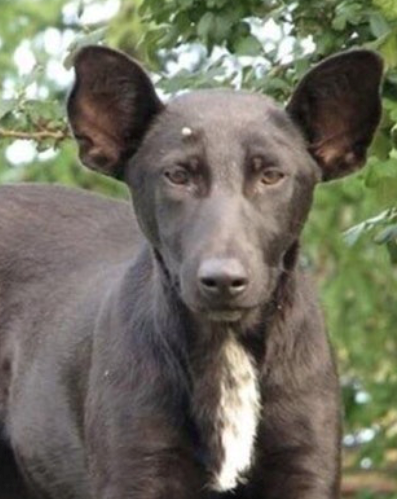
\includegraphics[width=0.5\columnwidth]{dog.png}
	\caption{Imagen original 1}
\end{figure}

\begin{figure}[h]
	\centering
	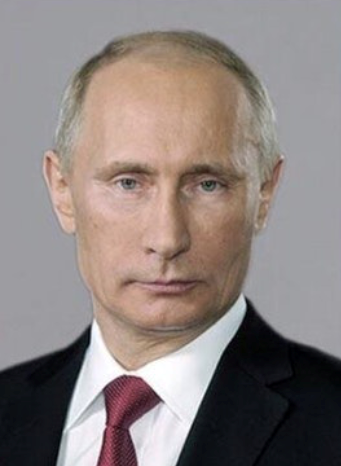
\includegraphics[width=0.5\columnwidth]{putin.png}
	\caption{Imagen original 2}
\end{figure}


\begin{figure}[h]
	\centering
	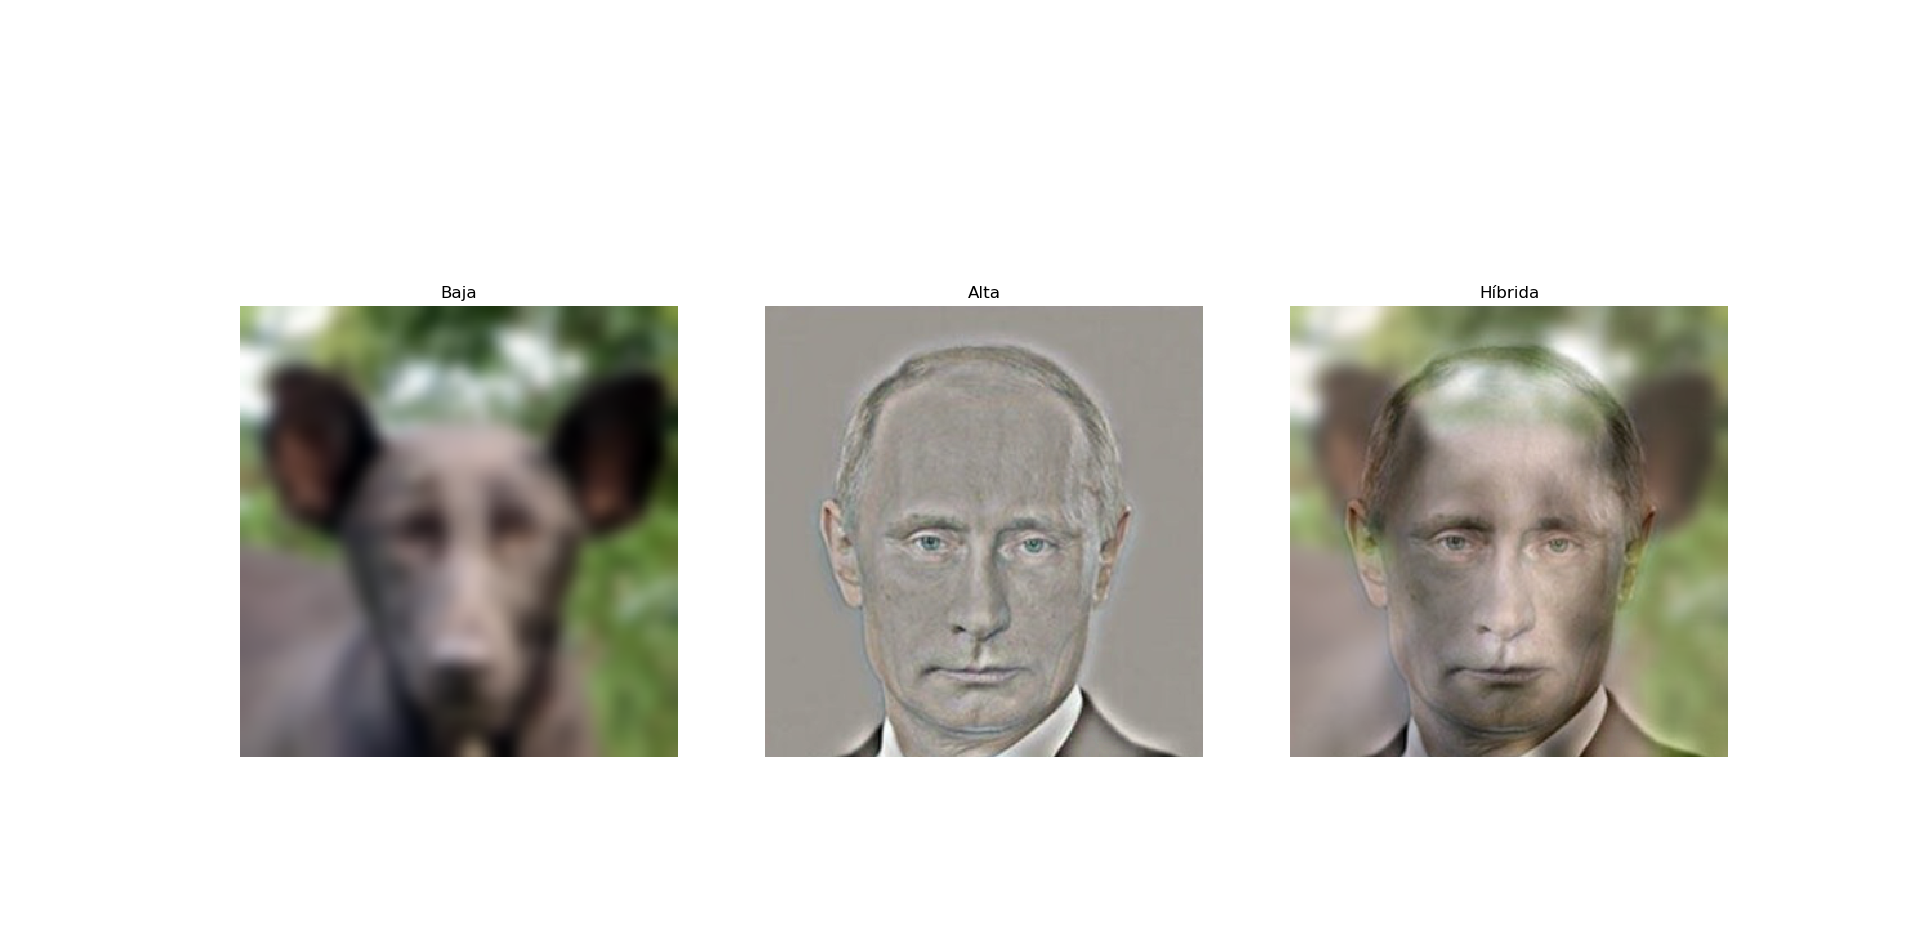
\includegraphics[width=1.0\columnwidth]{b3a.png}
	\caption{Imágenes baja/alta frecuencia e híbrida}

	\centering
	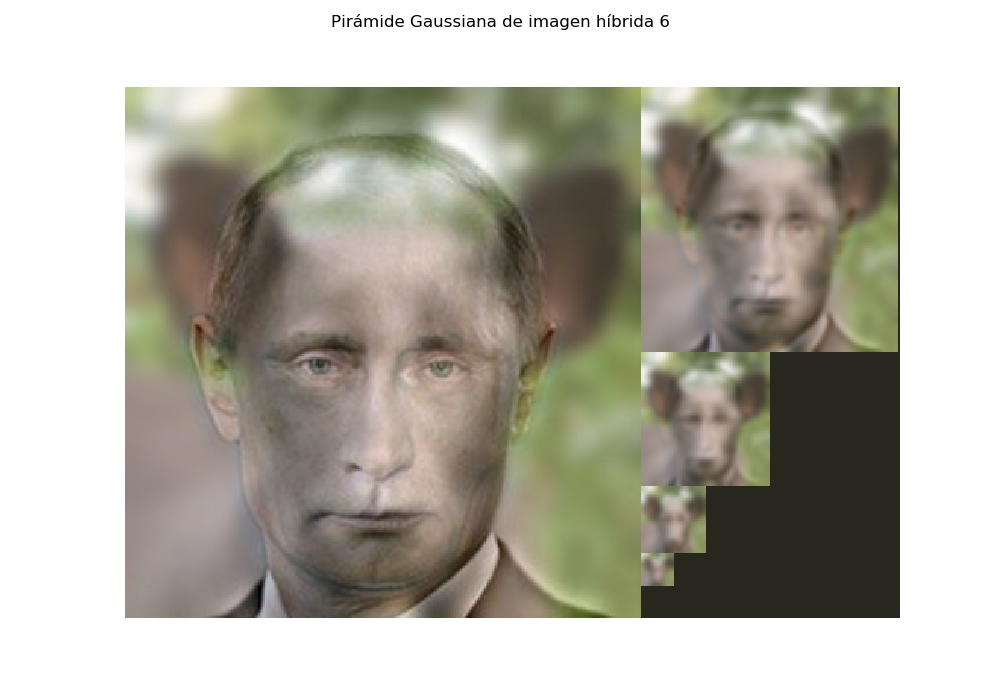
\includegraphics[width=1.0\columnwidth]{b3b.png}
	\caption{Pirámide Gaussiana de imágen híbrida}
\end{figure}

\end{document}